\documentclass[10pt,mathserif]{beamer}

\usepackage{graphicx,amsmath,amssymb,psfrag,mathtools}
\usepackage{soul}
\usepackage{amsmath,amsfonts,amsthm,bbm}
\usepackage{stmaryrd}
\usepackage{subcaption}



%Code block environment
\usepackage{listings}


\definecolor{lightgrey}{gray}{0.8}
\definecolor{medgrey}{gray}{0.6}
\definecolor{darkgrey}{gray}{0.4}
\usepackage{xcolor}
\lstset { %
    backgroundcolor=\color{black!5}, % set backgroundcolor
    basicstyle=\ttfamily,
    showstringspaces=false,
    commentstyle = \ttfamily,
    commentstyle=\color{commentgreen}\ttfamily,
    morecomment=[l][\color{darkgrey}]{//},
}



\usepackage{tikz}
\usetikzlibrary{matrix,chains,positioning,decorations.pathreplacing,arrows}
\usetikzlibrary{positioning,calc}
\usepackage{tkz-euclide}
%\usetkzobj{all}





%-------------------------------------------------------------------------------
%Definition of operator font
 \usepackage[bb=boondox]{mathalfa}
%% import \varmathbb without affecting other fonts
\usepackage{xparse}
\DeclareFontFamily{U}{ntxmia}{}
\DeclareFontShape{U}{ntxmia}{m}{it}{<-> ntxmia }{}
\DeclareFontShape{U}{ntxmia}{b}{it}{<-> ntxbmia }{}
\DeclareSymbolFont{lettersA}{U}{ntxmia}{m}{it}
\SetSymbolFont{lettersA}{bold}{U}{ntxmia}{b}{it}
\ExplSyntaxOn
\NewDocumentCommand{\varmathbb}{m}
 {
  \tl_map_inline:nn { #1 }
   {
    \use:c { varbb##1 }
   }
 }
\tl_map_inline:nn { ABCDEFGHIJKLMNOPQRSTUVWXYZ }
 {
  \exp_args:Nc \DeclareMathSymbol{varbb#1}{\mathord}{lettersA}{\int_eval:n { `#1+67 }}
 }
\exp_args:Nc \DeclareMathSymbol{varbbk}{\mathord}{lettersA}{169}
\ExplSyntaxOff
%%
\makeatletter
\DeclareFontFamily{U}{tipa}{}
\DeclareFontShape{U}{tipa}{m}{n}{<->tipa10}{}
\newcommand{\arc@char}{{\usefont{U}{tipa}{m}{n}\symbol{62}}}%

\newcommand{\arc}[1]{\mathpalette\arc@arc{#1}}

\newcommand{\arc@arc}[2]{%
  \sbox0{$\m@th#1#2$}%
  \vbox{
    \hbox{\resizebox{\wd0}{\height}{\arc@char}}
    \nointerlineskip
    \box0
  }%
}
\makeatother
\newcommand{\opA}{{\varmathbb{A}}}
\newcommand{\opB}{{\varmathbb{B}}}
\newcommand{\opC}{{\varmathbb{C}}}
\newcommand{\opD}{{\varmathbb{D}}}
\newcommand{\opE}{{\varmathbb{E}}}
\newcommand{\opF}{{\varmathbb{F}}}
\newcommand{\opG}{{\varmathbb{G}}}
\newcommand{\opH}{{\varmathbb{H}}}
\newcommand{\opI}{{\varmathbb{I}}}
\newcommand{\opJ}{{\varmathbb{J}}}
\newcommand{\opK}{{\varmathbb{K}}}
\newcommand{\opL}{{\varmathbb{L}}}
\newcommand{\opM}{{\varmathbb{M}}}
\newcommand{\opN}{{\varmathbb{N}}}
\newcommand{\opO}{{\varmathbb{O}}}
\newcommand{\opP}{{\varmathbb{P}}}
\newcommand{\opQ}{{\varmathbb{Q}}}
\newcommand{\opR}{{\varmathbb{R}}}
\newcommand{\opS}{{\varmathbb{S}}}
\newcommand{\opT}{{\varmathbb{T}}}
\newcommand{\opU}{{\varmathbb{U}}}
\newcommand{\opV}{{\varmathbb{V}}}
\newcommand{\opW}{{\varmathbb{W}}}
\newcommand{\opX}{{\varmathbb{X}}}
\newcommand{\opY}{{\varmathbb{Y}}}
\newcommand{\opZ}{{\varmathbb{Z}}}
\newcommand{\opZer}{\mathbb{0}}
%-------------------------------------------------------------------------------



%-------------------------------------------------------------------------------
%Definition of other font types
\newcommand{\va}{{\mathbf{a}}}
\newcommand{\vb}{{\mathbf{b}}}
\newcommand{\vc}{{\mathbf{c}}}
\newcommand{\vd}{{\mathbf{d}}}
\newcommand{\ve}{{\mathbf{e}}}
\newcommand{\vf}{{\mathbf{f}}}
\newcommand{\vg}{{\mathbf{g}}}
\newcommand{\vh}{{\mathbf{h}}}
\newcommand{\vi}{{\mathbf{i}}}
\newcommand{\vj}{{\mathbf{j}}}
\newcommand{\vk}{{\mathbf{k}}}
\newcommand{\vl}{{\mathbf{l}}}
\newcommand{\vm}{{\mathbf{m}}}
\newcommand{\vn}{{\mathbf{n}}}
\newcommand{\vo}{{\mathbf{o}}}
\newcommand{\vp}{{\mathbf{p}}}
\newcommand{\vq}{{\mathbf{q}}}
\newcommand{\vr}{{\mathbf{r}}}
\newcommand{\vs}{{\mathbf{s}}}
\newcommand{\vt}{{\mathbf{t}}}
\newcommand{\vu}{{\mathbf{u}}}
\newcommand{\vv}{{\mathbf{v}}}
\newcommand{\vw}{{\mathbf{w}}}
\newcommand{\vx}{{\mathbf{x}}}
\newcommand{\vy}{{\mathbf{y}}}
\newcommand{\vz}{{\mathbf{z}}}

\newcommand{\vA}{{\mathbf{A}}}
\newcommand{\vB}{{\mathbf{B}}}
\newcommand{\vC}{{\mathbf{C}}}
\newcommand{\vD}{{\mathbf{D}}}
\newcommand{\vE}{{\mathbf{E}}}
\newcommand{\vF}{{\mathbf{F}}}
\newcommand{\vG}{{\mathbf{G}}}
\newcommand{\vH}{{\mathbf{H}}}
\newcommand{\vI}{{\mathbf{I}}}
\newcommand{\vJ}{{\mathbf{J}}}
\newcommand{\vK}{{\mathbf{K}}}
\newcommand{\vL}{{\mathbf{L}}}
\newcommand{\vM}{{\mathbf{M}}}
\newcommand{\vN}{{\mathbf{N}}}
\newcommand{\vO}{{\mathbf{O}}}
\newcommand{\vP}{{\mathbf{P}}}
\newcommand{\vQ}{{\mathbf{Q}}}
\newcommand{\vR}{{\mathbf{R}}}
\newcommand{\vS}{{\mathbf{S}}}
\newcommand{\vT}{{\mathbf{T}}}
\newcommand{\vU}{{\mathbf{U}}}
\newcommand{\vV}{{\mathbf{V}}}
\newcommand{\vW}{{\mathbf{W}}}
\newcommand{\vX}{{\mathbf{X}}}
\newcommand{\vY}{{\mathbf{Y}}}
\newcommand{\vZ}{{\mathbf{Z}}}

\newcommand{\cA}{{\mathcal{A}}}
\newcommand{\cB}{{\mathcal{B}}}
\newcommand{\cC}{{\mathcal{C}}}
\newcommand{\cD}{{\mathcal{D}}}
\newcommand{\cE}{{\mathcal{E}}}
\newcommand{\cF}{{\mathcal{F}}}
\newcommand{\cG}{{\mathcal{G}}}
\newcommand{\cH}{{\mathcal{H}}}
\newcommand{\cI}{{\mathcal{I}}}
\newcommand{\cJ}{{\mathcal{J}}}
\newcommand{\cK}{{\mathcal{K}}}
\newcommand{\cL}{{\mathcal{L}}}
\newcommand{\cM}{{\mathcal{M}}}
\newcommand{\cN}{{\mathcal{N}}}
\newcommand{\cO}{{\mathcal{O}}}
\newcommand{\cP}{{\mathcal{P}}}
\newcommand{\cQ}{{\mathcal{Q}}}
\newcommand{\cR}{{\mathcal{R}}}
\newcommand{\cS}{{\mathcal{S}}}
\newcommand{\cT}{{\mathcal{T}}}
\newcommand{\cU}{{\mathcal{U}}}
\newcommand{\cV}{{\mathcal{V}}}
\newcommand{\cW}{{\mathcal{W}}}
\newcommand{\cX}{{\mathcal{X}}}
\newcommand{\cY}{{\mathcal{Y}}}
\newcommand{\cZ}{{\mathcal{Z}}}
%-------------------------------------------------------------------------------




%-------------------------------------------------------------------------------
%% macros for math notions and operators
\newcommand{\EE}{{\mathbb{E}}}
\newcommand{\expec}{\mathbb{E}}
\newcommand{\Prob}{{\mathrm{Prob}}} % probability

\newcommand{\reals}{\mathbb{R}}
\newcommand{\RR}{\mathbb{R}}
\newcommand{\complex}{\mathbb{C}}
\newcommand{\CC}{\mathbb{C}}
\newcommand{\nats}{\mathbb{N}}
\newcommand{\NN}{\mathbb{N}}
\newcommand{\ZZ}{\mathbb{Z}}
\newcommand{\bigO}{\mathcal{O}}
\newcommand{\order}[1]{{\mathcal{O}\left(#1\right)}}
\renewcommand{\SS}{{\mathbb{S}}}
\newcommand{\SSp}{\mathbb{S}_{+}}
\newcommand{\SSpp}{\mathbb{S}_{++}}
\newcommand{\sign}{\mathrm{sign}}
\newcommand{\vzero}{\mathbf{0}}
\newcommand{\vone}{{\mathbf{1}}}

\renewcommand{\Re}{\operatorname{Re}} 	%Real part
\renewcommand{\Im}{\operatorname{Im}}	%imaginary part

%\newcommand{\supp}{{\mathrm{supp}}} % support
\newcommand{\range}{\mathrm{range}\,} % domain
\newcommand{\tr}{{\mathrm{tr}}} % trace
%-------------------------------------------------------------------------------





%-------------------------------------------------------------------------------
%% Theorem definitions
\setbeamertemplate{theorems}[ams style] 
\newtheorem*{theorem*}{Theorem}
%\newtheorem{lemma}{Lemma}    % already provided by amsthm
\newtheorem{proposition}{Proposition}
%\newtheorem{proof}{Proof}  % already provided by amsthm


%-------------------------------------------------------------------------------
%% operator and convex analysis definitions

\newcommand*{\fix}{\mathrm{Fix}\,}
\newcommand*{\zer}{\mathrm{Zer}\,}
\newcommand*{\gra}{\mathrm{Gra}\,}
\newcommand{\prox}{\mathrm{Prox}}
\newcommand{\proj}{\Pi}
\newcommand{\aff}{\mathrm{aff}\,}    %affine hull
\newcommand{\intr}{\mathrm{int}\,}   %interior
\newcommand{\relint}{\mathrm{ri}\,}  %relative interior
\newcommand{\dom}{\mathrm{dom}\,} % domain
\newcommand{\epi}{\mathrm{epi}\,} % epigraph
\newcommand{\dist}{\mathrm{dist}}
\newcommand{\lagrange}{\mathbf{L}}  %saddle function
\newcommand{\fitzpatrick}{\mathbf{F}}   %Fitzpatrick function
\newcommand{\vecdelay}{\boldsymbol{d}}   %vector delay
\DeclareMathOperator*{\argmin}{argmin}
\DeclareMathOperator*{\argmax}{argmax}

%-------------------------------------------------------------------------------
%SRG definitions
\newcommand{\ereal}{\overline{\mathbb{R}^2}}
\newcommand{\ecomplex}{\overline{\mathbb{C}}}
\newcommand{\binfty}{{\boldsymbol \infty}}
\newcommand{\rarc}{\mathrm{Arc}^+}
\newcommand{\larc}{\mathrm{Arc}^-}


%-------------------------------------------------------------------------------




%-------------------------------------------------------------------------------
%Miscellaneous Stuff
%% sequences
\newcommand{\itom}{_{i=1}^{m}}
\newcommand{\ieqm}{i=1,\dots,m}

% use \numberthis to add an equation number in align*
\newcommand\numberthis{\addtocounter{equation}{1}\tag{\theequation}}

\newcolumntype{P}[1]{>{\centering\arraybackslash}p{#1}}

\mode<presentation>
{
\usetheme{default}
}
\setbeamertemplate{navigation symbols}{}
\usecolortheme[rgb={0.13,0.28,0.59}]{structure}
\setbeamertemplate{itemize subitem}{--}
\setbeamertemplate{frametitle} {
	\begin{center}
	  {\large\bf \insertframetitle}
	\end{center}
}

\newcommand\footlineon{
  \setbeamertemplate{footline} {
    \begin{beamercolorbox}[ht=2.5ex,dp=1.125ex,leftskip=.8cm,rightskip=.6cm]{structure}
      \footnotesize \insertsection
      \hfill
      {\insertframenumber}
    \end{beamercolorbox}
    \vskip 0.45cm
  }
}
\footlineon


\newcommand\footlineoff{
  \setbeamertemplate{footline} {
    \begin{beamercolorbox}[ht=2.5ex,dp=1.125ex,leftskip=.8cm,rightskip=.6cm]{structure}
      \footnotesize 
      \hfill
      {\insertframenumber}
    \end{beamercolorbox}
    \vskip 0.45cm
  }
}


\newcommand\blfootnote[1]{%
  \begingroup
  \renewcommand\thefootnote{}\footnote{#1}%
  \addtocounter{footnote}{-1}%
  \endgroup
}


\AtBeginSection[] 
{ 
	\begin{frame}<beamer> 
		\frametitle{Outline} 
		\tableofcontents[currentsection,currentsubsection] 
	\end{frame} 
} 

%% wotao's preference

        % itemize, black bullet, %150 spacing between items using "witemize"
        \newenvironment{witemize}{\itemize\addtolength{\itemsep}{0.3\baselineskip}}{\enditemize}

\iffalse
        % \setbeamertemplate{itemize items}[square]
        \setbeamertemplate{itemize items}{\textbullet}
        \setbeamercolor{itemize item}{fg=black}
        \setbeamercolor{itemize subitem}{fg=black}
        \setbeamercolor{itemize subsubitem}{fg=black}
        \setbeamercolor{enumerate item}{fg=black}
        \setbeamercolor{enumerate subitem}{fg=black}
        \setbeamercolor{enumerate subsubitem}{fg=black}
        \setbeamertemplate{itemize/enumerate body begin}{\normalsize}
        \setbeamertemplate{itemize/enumerate subbody begin}{\normalsize}
        \setbeamertemplate{itemize/enumerate subsubbody begin}{\normalsize}

        % itemize enumerate use normal sized texts
        \setbeamertemplate{itemize/enumerate body begin}{\normalsize}
        \setbeamertemplate{itemize/enumerate subbody begin}{\normalsize}
        \setbeamertemplate{itemize/enumerate subsubbody begin}{\normalsize}

        % block, black over gray with no shadow
        \setbeamertemplate{blocks}[rounded][shadow=false]
        \setbeamercolor{block title}{fg=black,bg=gray!40}
        \setbeamercolor{block body}{fg=black,bg=gray!10}
\fi

\author{Ernest K. Ryu and Wotao Yin}

\date{Large-Scale Convex Optimization via Monotone Operators}


\title{\large \bfseries Asynchronous Coordinate Update Methods}

\begin{document}

\frame{
\thispagestyle{empty}
\titlepage
}

\begin{frame}{Background}
    \begin{itemize}
        \item Multi-core CPUs are common. To use CPU cores, we hope to parallelize coordinate updates 
        \item Since (block) coordinates can depend on each other, their parallel updates need to exchange information
        \item  Roughly speaking, if an update can compute without waiting for the latest information from the others, we call it asynchronous
        \item Asynchronism is important to the efficiency of parallel computing
        \item Without asynchronism, all updates would have to wait for the arrival of latest information, so the speed of parallel updates would be dictated by the slowest core, the most difficult update, and the longest communication delay
        \item This chapter introduces an asynchronous coordinate update method and analyzes its convergence
        \item Terminology: we call CPU core ``computational agent'' or ``agent''
    \end{itemize}
\end{frame}

\begin{frame}[fragile]
\frametitle{Coordinate partitioning}
Let $\opT\colon\reals^n\rightarrow\reals^n$ be $\theta$-averaged with $\opT=\opI-\theta\opS$.

Partition $x= (x_1,\dots,x_m)\in \reals^n$ and 
\[
\opT(x)=\begin{bmatrix}
(\opT(x))_1\\
\vdots\\
(\opT(x))_i\\
\vdots\\
(\opT(x))_m
\end{bmatrix}
\qquad
\begingroup
\renewcommand*{\arraystretch}{.8}
\opT_i(x)=\begin{bmatrix}
x_1\\
\vdots\\
x_{i-1}\\
(\opT(x))_i\\
x_{i+1}\\
\vdots\\
x_m
\end{bmatrix}
\endgroup
\qquad
\opS _i(x)=
\begin{bmatrix}
0\\
\vdots\\
0\\
(\opS (x))_i\\
0\\
\vdots\\
0
\end{bmatrix}.
\]
We begin with a standard synchronous implementation of
\begin{align*}
  x^{k+1} = x^k - \eta \opS x^k,
\end{align*}
on multiple computational agents.

\end{frame}

\begin{frame}[plain,fragile]
\frametitle{Synchronous parallel FPI}
Multiple agents simultaneously run:
\begin{lstlisting}
// p agents run while loop simultaneously
// x and s are vectors in shared memory
WHILE (not converged)
  1. WHILE (not all indices claimed)
       Claim index i not yet claimed
       Read x
       Write s[i] = eta*S[i](x)
  2. Synchronize: wait for all agents
  -----------------------------------------------
  3. WHILE (not all indices claimed)
       Claim index i not yet claimed
       Write x[i] = x[i] - s[i]
  4. Synchronize: wait for all agents
  -----------------------------------------------
\end{lstlisting}
%This algorithm (deterministically) computes the iteration $x^{k+1}=x^k - \eta \opS x^k$.
Steps 2, 4 are \emph{synchronization barriers}. Algorithm is \emph{synchronous parallel}.
\end{frame}




\begin{frame}[fragile]
\frametitle{Synchronization}
\begin{lstlisting}
WHILE (not converged)
  1. WHILE (not all indices processed)
       Read x
       Write s[i] = eta*S[i](x)
  2. Synchronize: wait for all agents
  -----------------------------------------------
  3. WHILE (not all indices processed)
       Write x[i] = x[i] - s[i]
  4. Synchronize: wait for all agents
  -----------------------------------------------
\end{lstlisting}
At any time, the agents are either all in Steps 1--2 or all in Steps 3--4.
\begin{itemize}
\item Step 1 reads \verb|x|, does not write to \verb|x|. Step 3 reads \verb|x|, writes to \verb|x|.
\item Step 2 prevents agents finished with Step 1 from proceeding to Step 3 and changing \verb|x| while the other agents are still using \verb|x| in Step 1.
\item Step 4 prevents agents finished with Step 3 from proceeding to Step 1 and reading \verb|x| while other agents are still changing \verb|x|.
\end{itemize}
\end{frame}



\begin{frame}{Cost of synchrony}

As the number of computing agents grows, the cost of synchrony becomes significant.

\bigskip

Faster agents must wait idly for the slower ones.

\bigskip

The synchronization barrier is itself an algorithm with a cost.

\bigskip

Communication congestion is another cost that can occur when multiple agents simultaneously write data in Steps 1 and 3.

\end{frame}



\begin{frame}[fragile]
\frametitle{Asynchronous parallelism}
An algorithm is \emph{asynchronous parallel} if it avoids synchronization barriers. 

\medskip

Simply removing the synchronization barriers, however, does not work.
\bigskip

Naive barrier--free algorithm:
\begin{lstlisting}
// p agents run the while loop asynchronously
// x and s are vectors in shared memory
WHILE (not converged)
  1. Select i from Uniform{1,2,...,m}
  2. Read x
  3. Compute s[i] = eta*S[i](x)
  4. Write x[i] = x[i] - s[i] //Incorrect!
\end{lstlisting}
Now, agents run completely uncoordinated, and the cost of synchronization is eliminated.
\medskip

Now, the number of updates is determined by total computing power, rather than the slowest agent.
\end{frame}



\begin{frame}[fragile]
\frametitle{Stale information}

\begin{lstlisting}
// p agents run the while loop asynchronously
// x and s are vectors in shared memory
WHILE (not converged)
  1. Select i from Uniform{1,2,...,m}
  2. Read x
  3. Compute s[i] = eta*S[i](x)
  4. Write x[i] = x[i] - s[i] //Incorrect!
\end{lstlisting}
However, the algorithm does \emph{not} work. It is neither the FPI $x^{k+1}=(\opI-\eta \opS)x^k$ nor the RC-FPI $x^{k+1}=(\opI-\eta \opS_{i(k)})x^k$.
\medskip

When an agent performs Step 4, other agents may have updated \verb|x|, rendering \verb|x| used to compute Step 3 outdated. In this case, we say \verb|x| is \emph{stale}. Step 4 does
\[
x^{k+1}=x^k-\eta \opS_{i(k)}\hat{x}^k
\]
where $\hat{x}^k$ contains information \emph{older than} $x^k$.
\medskip

Asynchrony must be carefully considered and designed around.
\end{frame}

\section{Asynchronous fixed-point iteration}


\begin{frame}[fragile,plain]
\frametitle{Asynchronous coordinate-update fixed-point iteration}

We can account for staleness if we enforce \emph{exclusive access} in Step 4.\\
An agent has exclusive access to \verb|x| in shared memory if no other agent can read from or write to \verb|x| simultaneously.




\vspace{0.1in}
\emph{Asynchronous coordinate-update fixed-point iteration} (AC-FPI) with an \emph{operational definition}:
\begin{lstlisting}
// p agents run the while loop asynchronously
// x is a vector stored in shared memory
WHILE (not converged)
  1. Select i from Uniform{1,2,...,m}
  2. Read x
  3. Compute s[i] = eta*S[i](x)
  4. Exclusively read x[i] and
                 write x[i] = x[i] - s[i]
\end{lstlisting}
While an agent is updating \verb|x[i]| in Step 4, others cannot access \verb|x[i]|.
\vspace{0.1in}

If $(\opS x)_i$ depends on only some blocks of $x$, an agent running Step 2 needs to read only those of \verb|x|, unaffected by any exclusive access on the other blocks of \verb|x| caused by other agents running Step 4 simultaneously.
\end{frame}


\begin{frame}[fragile]
\frametitle{Benefit of asynchrony}
\begin{lstlisting}
// p agents run the while loop asynchronously
// x is a vector stored in shared memory
WHILE (not converged)
  1. Select i from Uniform{1,2,...,m}
  2. Read x
  3. Compute s[i] = eta*S[i](x)
  4. Exclusively read x[i] and
                 write x[i] = x[i] - s[i]
\end{lstlisting}
AC-FPI removes explicit synchronization barriers, though it still requires exclusive access in writing to $\verb|x[i]|$.




\vspace{0.1in}

When there are much more blocks than agents, i.e., $p\ll m$, it is rare for an agent to wait for the release of a block's exclusive access; hence, most, albeit not all, idle time is eliminated.
\end{frame}


\begin{frame}[fragile,plain]
\frametitle{Defining ``iterates''}

To analyze AC-FPI, we need a \emph{mathematical definition}:
%We present one here, and Exercise \ref{exercise:afterread} presents another.
\begin{itemize}
\item
$x^0$ is the state of \verb|x| before the start of the algorithm.
\item 
The $k$th iterate is $x^k=(x_1^k,\dots,x_m^k)$.
\item 
Iteration count increments by $1$ when an agent completes an update of \verb|x| in global memory, i.e., when an agent completes Step 4.
\item 
When the iteration counter becomes $k$, if no agent is writing to \verb|x[j]| then $x_j^k$ is the state of \verb|x[j]| at that time.
\item 
When the iteration counter becomes $k$, if an agent is updating \verb|x[j]| then $x_j^k$ is what \verb|x[j]| used to be right before the agent currently writing to the block started the update.
% \begin{itemize}
%     \item  If updates of Step 4 do not overlap in time (possible if Step 3 takes very long and there are few agents) then $x^k$ is precisely the state of \verb|x| when the iteration counter increments.
% \end{itemize}
\item
If two or more agents finish updating different blocks at the same time, we break the tie arbitrarily.
% \begin{itemize}
%     \item Exclusive access prevents multiple agents from concurrently updating the same block, but different agents may concurrently update different blocks.
% \end{itemize}
\end{itemize}
\vspace{0.1in}


(There are other valid approaches to defining the iterates. See exercises.)

\vspace{0.1in}



\end{frame}


\begin{frame}[plain]
% \vspace{-0.1in}
\begin{center}
    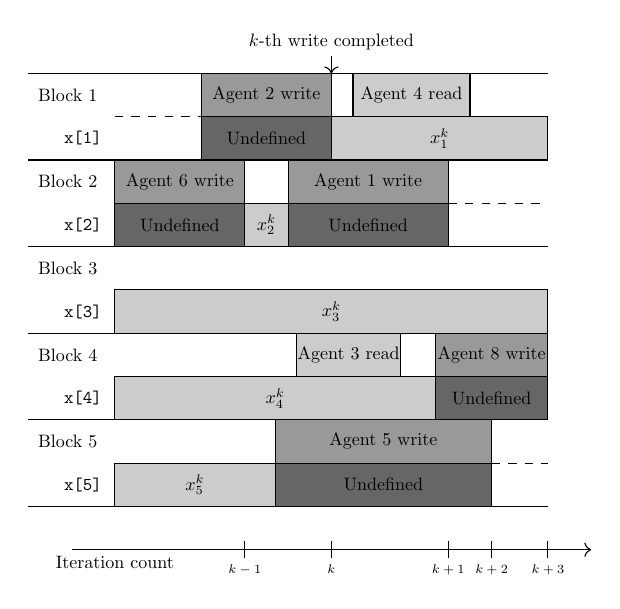
\begin{tikzpicture}[scale = 0.55, every node/.style={scale=0.65}]
    
    \node[above] at (5,7.4) {$k$-th write completed};

\draw[->] (5,7.4) -- (5,7);

        
\node[text width=3cm] at (0.0,-1.5) {Block 5};
\node[text width=3cm] at (0.0,0.5) {Block 4};
\node[text width=3cm] at (0.0,2.5) {Block 3};
\node[text width=3cm] at (0.0,4.5) {Block 2};
\node[text width=3cm] at (0.0,6.5) {Block 1};


\node[text width=3cm] at (0.6,-2.5) {\texttt{x[5]}};
\node[text width=3cm] at (0.6,-0.5) {\texttt{x[4]}};
\node[text width=3cm] at (0.6,1.5) {\texttt{x[3]}};
\node[text width=3cm] at (0.6,3.5) {\texttt{x[2]}};
\node[text width=3cm] at (0.6,5.5) {\texttt{x[1]}};

\def\n{-2};
\def\m{10};
\draw (\n, -3) -- (\m, -3);
\draw (\n, -1) -- (\m, -1);
\draw (\n, 1) -- (\m, 1);
\draw (\n, 3) -- (\m, 3);
\draw (\n, 5) -- (\m, 5);
\draw (\n, 7) -- (\m, 7);

\def\n{0};
\draw[style=dashed] (8.7, -2) -- (\m, -2);
%\draw[style=dashed] (\n, 0) -- (\m, 0);
%\draw[style=dashed] (\n, 2) -- (\m, 2);
\draw[style=dashed] (7.7, 4) -- (\m, 4);
\draw[style=dashed] (\n, 6) -- (2, 6);

%\node[style=rectangle,draw = black] at (1,0) {Agent 2 write};
\draw[fill=medgrey] (2,6) rectangle (5,7) node[pos=.5] {Agent 2 write};
\draw[fill=lightgrey] (5.5,6) rectangle (8.2,7) node[pos=.5] {Agent 4 read};
\draw[fill=medgrey] (0,4) rectangle (3,5) node[pos=.5] {Agent 6 write};
\draw[fill=medgrey] (4,4) rectangle (7.7,5) node[pos=.5] {Agent 1 write};
%\draw[fill=medgrey] (1.2,0) rectangle (4.,1) node[pos=.5] {Agent 4 write};
\draw[fill=lightgrey] (4.2,0) rectangle (6.6,1) node[pos=.5] {Agent 3 read};
\draw[fill=medgrey] (7.4,0) rectangle (10,1) node[pos=.5] {Agent 8 write};
\draw[fill=medgrey] (3.7,-2) rectangle (8.7,-1) node[pos=.5] {Agent 5 write};

\draw[fill=lightgrey] (5,5) rectangle (10,6) node[pos=.5] {$x_1^k$};
\draw[fill=darkgrey] (2,5) rectangle (5,6) node[pos=.5] {Undefined};
%\draw[fill=lightgrey] (1,5) rectangle (2,6) node[pos=.5] {$x_1^{k-1}$};

\draw[fill=darkgrey] (0,3) rectangle (3,4) node[pos=.5] {Undefined};
\draw[fill=lightgrey] (3,3) rectangle (4,4) node[pos=.5] {$x_2^k$};
\draw[fill=darkgrey] (4,3) rectangle (7.7,4) node[pos=.5] {Undefined};
%\draw[fill=lightgrey] (7.7,3) rectangle (10,4) node[pos=.5] {$x_2^{k+1}$};

\draw[fill=lightgrey] (0,1) rectangle (10,2) node[pos=.5] {$x_3^k$};

\draw[fill=lightgrey] (0,-1) rectangle (7.4,0) node[pos=.5] {$x_4^k$};
\draw[fill=darkgrey] (7.4,-1) rectangle (10,0) node[pos=.5] {Undefined};


\draw[fill=darkgrey] (3.7,-3) rectangle (8.7,-2) node[pos=.5] {Undefined};
\draw[fill=lightgrey] (0,-3) rectangle (3.7,-2) node[pos=.5] {$x_5^k$};

\draw[->] (-1,-4) -- (11,-4);
\draw (0,-4) node[below]{Iteration count};

\def\k{3};
\draw ({\k},-3.8)  -- ({\k},-4.2);
\draw ({\k},-4.2) node[below] {\scriptsize $k-1$};

\def\k{5};
\draw ({\k},-3.8)  -- ({\k},-4.2);
\draw ({\k},-4.2) node[below] {\scriptsize $k$};

\def\k{7.7};
\draw ({\k},-3.8)  -- ({\k},-4.2);
\draw ({\k},-4.2) node[below] {\scriptsize $k+1$};

\def\k{8.7};
\draw ({\k},-3.8)  -- ({\k},-4.2);
\draw ({\k},-4.2) node[below] {\scriptsize $k+2$};

\def\k{10};
\draw ({\k},-3.8)  -- ({\k},-4.2);
\draw ({\k},-4.2) node[below] {\scriptsize $k+3$};



    \end{tikzpicture}
    \end{center}
% \vspace{-0.1in}
    
In this illustration, $x^k$ is defined when Agent 2 completes writing to Block 1.
Since Blocks 3 and 4 are not being updated, 
$x_3^k$ and $x_4^k$ are the state of \texttt{x[3]} and \texttt{x[4]} at the time.
Since Blocks 2 and 5 are being updated, 
$x_2^k$ and $x_5^k$ are the state of \texttt{x[2]} and \texttt{x[5]} before the writes had begun.
\end{frame}


\begin{frame}[fragile]
\frametitle{Delay notation of staleness}

Write $i(k)$ for the index of the $k$th update.
Again consider the IID random coordinate selection rule for simplicity.

\vspace{0.1in}

The value of \verb|x| that an agent has read in AC-FPI Step 2 may become stale by the time the agent performs Step 4.
Write $\hat{x}^k$ for the stale value of $\verb|x|$ used for the update of $x^k$ to $x^{k+1}$, i.e., $x^{k+1}=x^k-\eta \opS_{i(k)}\hat{x}^k$.
\vspace{0.1in}

It is possible that $\hat{x}^k\ne x^\ell$ for any $\ell=0,\dots,k$ since other agents can update blocks while $\hat{x}^k$ is being read block-by-block in Step 2.
The exclusive access of Step 4 is on the block \verb|x[i]|, not on the entire \verb|x|.

\vspace{0.1in}

Consider a coordinate-by-coordinate notion of staleness:
\begin{align*}
  \hat{x}^k & =\big( x_1^{k-d_1(k)},\dots,x_m^{k-d_m(k)}\big),
\end{align*}
to denote that the $i$th block of $\hat{x}^k$ is outdated by $d_i(k)\ge 0$ iterations.
$d_1(k),\dots,d_m(k)$ are the \emph{block delays}, and
\[
\vecdelay(k)=(d_1(k),\dots,d_m(k)) \in\mathbb{N}^m_+
\]
is the \emph{vector delay}. Write $\hat{x}^k=x^{k-\vecdelay(k)}$.
\end{frame}


\begin{frame}
\frametitle{Mathematical definition of the AC-FPI}
Mathematical definition of the AC-FPI:
\begin{equation}\label{eq:ac_fpi}
x^{k+1}=x^k-\eta \opS_{i(k)}x^{k-\vecdelay(k)}.
\end{equation}
\vspace{0.1in}

AC-FPI is a stochastic algorithm realized by the random variables $i(0),i(1),\dots$ and $\vecdelay(0),\vecdelay(1),\dots$.
\vspace{0.1in}

Randomness of $i(0),i(1),\dots$ is injected by design.
Randomness of $\vecdelay(0),\vecdelay(1),\dots$ comes from the randomness of $i(0),i(1),\dots$ and the randomness of the agents' computation time.
\end{frame}






\begin{frame}
\frametitle{ARock and convergence of the AC-FPI}
The AC-FPI update $x^{k+1}=x^k-\eta \opS_{i(k)}x^{k-\vecdelay(k)}$ models many asynchronous algorithms considered in the literature.
% but not the ones without the exclusive access of Step 4 or other measures to prevent inconsistent reads, which we discuss in \S\ref{ss:race_cond}.
% We broadly refer to all such methods as instances of the AC-FPI.

\vspace{0.2in}

We analyze an instance of AC-FPI with the \emph{ARock assumptions}:
\begin{itemize}
    %\item the iterates are defined by $x^{k+1}=x^k-\eta \opS_{i(k)}x^{k-\vecdelay(k)}$,
    \item $i(0),i(1),\dots$ are IID with uniform probability, 
    \item $i(k)$ and $\vecdelay(\ell)$ are independent for  $k=0,1,\dots$ and $\ell\le k$, and
    \item $\vecdelay(0),\vecdelay(1),\dots$ is a stochastic process %identically distributed and the distribution satisfies 
    %Assume that there exist $D$ and a nonincreasing sequence $Q_\ell\in[0,1]$, $\ell=0,1,\dots,$ such that $Q_\ell =0$ for $\ell>D$ and, for every $k=0,1,\dots$,
    with nonincreasing $Q_0,Q_1,\ldots\in[0,1]$ such that for every $k=0,1,\dots$,
    \begin{align}
        &\Prob\left[\max_{i=1,\dots,m} d_i(k) \ge \ell 
        \,\bigg|\,
        \vecdelay(k-1),\dots,\vecdelay(0),i(k-1),\dots,i(0)
        \right]\le Q_\ell,\nonumber\\
        %\text{and}\quad
        &\qquad\qquad\sum_{\ell=1}^{\infty}\ell (Q_\ell)^{1/2} < \infty.\label{eq:Plbnd}
      \end{align}
      This summability assumption is very mild. (C.f. Exercise~6.2.)
    %   See Exercise~\ref{exercise:delay_condition}.
      %In particular, it is satisfied if the random variables $\max_{i=1,\dots,m} d_i(k)$ for $k=0,1,\dots$ share a finite bound on their $(5+\varepsilon)$th moments for any $\varepsilon>0$. 
% \item
% The delays satisfy
% \begin{equation}
% \Prob\left[\vecdelay(k)=0\,|\,\vecdelay(k-1),\dots,\vecdelay(0),i(k-1),\dots,i(0)\right]>p_0>0\qquad
% \label{eq:mixing_assump}
% \end{equation}
% for all $k=0,1,\dots$. 
% In other words, there is always a  probability of at least $p_0$ that the delay is $0$.
% While this assumption is likely not necessary, it does simplify the proof.
\end{itemize}
\end{frame}


\begin{frame}
\setcounter{theorem}{2}
\frametitle{Convergence of AC-FPI}
\begin{theorem}
\label{thm:ac-fpi}
Assume $\opS\colon\reals^n\rightarrow\reals^n$ is $(1/2)$-cocoercive or, equivalently, that $\opT=\opI-\theta \opS$ is $\theta$-averaged with $\theta\in(0,1)$. Assume $\fix \opT\ne \emptyset$.
%Assume the random indices $i(0),i(1),\dots\in \{1,\dots,m\}$ are independent and identically distributed with probability $\Prob[i(k)=i]=p_i$ like in AC-FPI.
% Assume $i(0),i(1),\dots\in \{1,\dots,m\}$ and $\vecdelay(0),\vecdelay(1),\dots\in \mathbb{N}^m$ are independent.
% Assume $i(0),i(1),\dots$ are identically distributed with uniform probability.
% Assume $\vecdelay(0),\vecdelay(1),\dots$ satisfy the aforementioned assumptions.
Under the ARock assumptions, the AC-FPI $x^{k+1}=x^k-\eta \opS_{i(k)} x^{k-\vecdelay(k)}$ with any starting point $x^0\in \reals^n$ and step size $\eta$ obeying
\begin{align*}
  0<\eta<\left(1+\frac{2}{\sqrt{m}}\sum_{\ell=1}^{\infty}Q_\ell^{1/2}\right)^{-1}
\end{align*}
converges to one fixed point with probability 1, i.e.,
\[
x^k\rightarrow x^\star\quad\text{for some}~ x^\star\in \fix \opT
\]
holds with probability 1.
%For simplicity, let $(p_1,\dots,p_n) = (\frac{1}{n},\dots,\frac{1}{n})$.
 % with its tail probability obeying $\sum_{\ell=1}^{\infty}(\ell Q_\ell)^{1/2}<\infty$.
%The quantities
%$ \expec \dist^2(x^{k},\fix T)$,
%$\expec\|Tx^{k}-x^k\|^2$,
%and
%$\expec\|x^{k}-x^\star\|^2$  for any $x^\star\in \fix T$ decrease monotonically with $k$.
Furthermore, with probability 1,
\[
\dist(x^{k},\fix \opT)
%\stackrel{\mathrm{a.s.}}{\rightarrow}
\rightarrow
0.
\]
\vspace{-0.25in}
%and
%\begin{align*}
%\expec\|x^{k+1}-x^k\|^2\le \frac{\theta m}{(k+1)(1-\theta)}\dist^2(x^{0},\fix T).
%\end{align*}
\end{theorem}
\end{frame}


\begin{frame}
\frametitle{Discussion on stepsize and staleness}
For the stepsize
\begin{align*}
  0<\eta<\left(1+\frac{2}{\sqrt{m}}\sum_{\ell=1}^{\infty}Q_\ell^{1/2}\right)^{-1},
\end{align*}
given a fixed distribution of delays, i.e., fixed values of $Q_0,Q_1,\dots$, larger $m$ is \emph{more favorable}.
That is, the staleness becomes less harmful as the number of blocks grows.
If $m\rightarrow \infty$ with fixed $Q_0,Q_1,\dots$, the stepsize requirement becomes the same as that of Theorem~2.


\vspace{0.2in}

In practice, staleness may slow down AC-FPI.
Therefore, RC-FPI and AC-FPI represent a trade-off between better and faster iterations.
\end{frame}



\begin{frame}
\frametitle{Discussion of assumptions: Exclusive access}
In the operational definition of the AC-FPI, Step 4 requires exclusive access.
Otherwise, we would not be able to use the notation
\[
\hat{x}^k =x^{k-\vecdelay(k)}= (x_1^{k-d_1(k)},\dots,x_m^{k-d_m(k)}),
\]
as an agent can read a block while another agent is halfway through writing to the same block.



\end{frame}



\begin{frame}[fragile,plain]
\frametitle{Discussion of assumptions: Independence}

\begin{itemize}
    \item 
    We do assume that the sequence $i(0),i(1),\dots$ is IID.
    When index \verb|i| is sampled in Step 1 of the AC-FPI, we do not yet know which iteration count $k$ the index will be associated with.
    If the computational cost of each block is equal, then the IID sampling of Step 1 makes $i(0),i(1),\dots$ an IID sequence.
    \begin{itemize}
        \item 
        If the blocks have non-uniform computational costs, the choice of index affects the iteration count the update is assigned to and the IID assumption is violated.
        For example, if the $j$th block takes longer to compute, then $i(0)=j$ will have a lower probability than, say, $i(1000)=j$.
    \end{itemize}
    \item 
    We do assume that $i(k)$ and $\vecdelay(k)$ are independent for $k=0,1,\dots$.
    This is realistic if the computational costs of the blocks are uniform.
    \begin{itemize}
        \item 
        On the other hand, if, for example, the $j$th block is much more expensive to compute than others and $i(k)=j$, then it is likely that $\vecdelay(k)$ contains large delays.
    \end{itemize}
\end{itemize}
Removing these assumption makes the analysis much more difficult and leads to weaker results.
\end{frame}


\begin{frame}{Discussion of assumptions: dependence allowed}
    \begin{itemize}
        \item 
        We do not assume $\vecdelay(0),\vecdelay(1),\dots$ is an independent sequence.
        %; it usually is a dependent sequence.
        \begin{itemize}
            \item 
            It is likely that $\hat{x}^k$ and $\hat{x}^{k+1}$ are read at close points in time, and this makes $\vecdelay(k)$ and $\vecdelay(k+1)$ highly correlated.
        \end{itemize}
        \item 
        We do not assume $i(k)$ and $\vecdelay(\ell)$, $\ell>k$, are independent.
        \begin{itemize}
            \item 
            For example, if $i(k)=j$, then $d_j(k+1)>0$ is very likely.
        \end{itemize}
    \end{itemize}

    Even when the computational costs of the blocks are uniform, it is unrealistic to make these independence assumptions.
\end{frame}



\begin{frame}
\frametitle{Discussion of assumptions: Delays}
A common assumption in the literature is that the delays are bounded:
$$\max\{d_1(k),\dots,d_m(k)\}\le D\quad\text{for }k=0,1,\dots$$ for some $D<\infty$.
We do not make this assumption.

% While this bounded-delay assumption would simplify Stage 2 of our proof of Theorem~\ref{thm:ac-fpi}, it is not necessary.
% Therefore, we do not make this assumption. 
\end{frame}




\begin{frame}
\frametitle{Proof of Theorem~3}
%The proof is divided into stages. Since every iterate $x^k$ is a coordinate update from the previous iterate, we use the same definitions of total expectation $\EE$ and conditional expectation $\EE_{i(k)}$ as they are in the proof of Theorem \ref{thm:stochastic-iter}.
Write $\EE$ for the total expectation.
\vspace{0.1in}

Write $\EE_{i(k)}$ for the expectation over $i(k)$ conditioned on $\vecdelay(k),\dots,\vecdelay(0),i(k-1),\dots,i(0)$.

\vspace{0.1in}


Write
$\EE_{\vecdelay(k)}$ for the expectation over $\vecdelay(k)$ conditioned on $\vecdelay(k-1),\dots,\vecdelay(0),i(k-1),\dots,i(0)$.

\vspace{0.1in}

Write $\EE_{i(k),\vecdelay(k)}$ for the expectation over $i(k)$ and $\vecdelay(k)$ conditioned on $\vecdelay(k-1),\dots,\vecdelay(0),i(k-1),\dots,i(0)$.



\vspace{0.1in}

Note that the random variables $\vecdelay(k-1),\dots,\vecdelay(0),i(k-1),\dots,i(0)$ completely determine $x^{k},\dots,x^1$.
%Remember that $x^{k+1}$ is a random variable that depends on $x^k$, $i(k)$, and $\vecdelay(k)$.

\bigskip

The proof is divided into three stages.

\end{frame}




\begin{frame}
\frametitle{Proof of Theorem~3: Stage 1} 
Define the Lyapunov function
%such that they are nonnegative by design and has a monotonically-decreasing conditional expectation. For any fixed , we define
\begin{align*}
  V^k = \|x^k - x^\star\|^2 + \frac{1}{m}\sum_{d=1}^{\infty}c_d \|x^{k-d+1}-x^{k-d}\|^2,
\end{align*}
where $x^\star\in\fix\opT$ and $x^{0}=x^{-1}=x^{-2}=\cdots$.
Coefficients $c_d\ge 0$ will be determined later.
Clearly, $V^k\ge 0$.
We have $V^k<\infty$ since the sum is finite for a fixed $k<\infty$.
% As an aside, if one assumes the delays are bounded, the infinite sum can be replaced with a finite sum.
%As $k\to\infty$, the issue of summability arises.
% to the term $c_k\|x^1-x^0\|^2$, and 
\vspace{0.1in}

We show the key inequality
\begin{align}
  \EE_{i(k),\vecdelay(k)} V^{k+1} 
%  \le V^k - \frac{\eta}{m}\left(1-\eta -\frac{c_1\eta}{m}-\eta\sum_{d=1}^{{\tau}(k)}\varepsilon_d^{-1}\right)\EE_{\vecdelay(k)}\|\opS x^{k-\vecdelay(k)}\|^2. \label{eq:asymon}
   \le V^k - \frac{\eta}{m}\left(1 - \eta\left( 1 + \frac{2}{\sqrt{m}} \sum_{d=1}^{\infty}Q_d^{1/2}\right)\right)\EE_{\vecdelay(k)}\|\opS x^{k-\vecdelay(k)}\|^2.\label{eq:asymon}
\end{align}
(To skip the details of Stage 1, skip the next six slides.)
\end{frame}



%The early part of the proof of Theorem \ref{thm:stochastic-iter} up to \eqref{eq:stoxepd} still applies here except that we let $\eta \opS_{i(k)}x^{k-\vecdelay(k)}$ replace $\theta \opS_{i(k)}{x}^k$. In particular,

%We compute $\EE_{i(k)}\|x^{k+1} - x^\star\|^2$ to $\|x^k - x^\star\|^2$.



\begin{frame}
Mathematical definition of AC-FPI gives us
\begin{align*}
  \|x^{k+1} - x^\star\|^2 & = \|x^k - \eta \opS_{i(k)} x^{k-\vecdelay(k)} - x^\star\|^2 \nonumber\\
  & = \|x^k - x^\star\|^2 - 2\eta\langle \opS_{i(k)} x^{k-\vecdelay(k)} ,x^k - x^\star\rangle + \eta^2 \|\opS_{i(k)} x^{k-\vecdelay(k)}\|^2.
\end{align*}
Independence between $i(k)$ and $\vecdelay(k)$ gives us
\begin{align*}
  \EE_{i(k)} \opS_{i(k)} x^{k-\vecdelay(k)}= \frac{1}{m} \opS x^{k-\vecdelay(k)},\quad \EE_{i(k)} \|\opS_{i(k)} x^{k-\vecdelay(k)}\|^2 = \frac{1}{m} \|\opS x^{k-\vecdelay(k)}\|^2
\end{align*}
and
\begin{align}
  \EE_{i(k)}\|x^{k+1} - x^\star\|^2 & = \|x^k - x^\star\|^2 - \frac{2\eta}{m}\langle \opS x^{k-\vecdelay(k)} ,x^k - x^\star\rangle + \frac{\eta^2}{m} \|\opS x^{k-\vecdelay(k)}\|^2.\label{eq:exp1}
\end{align}
Using $(1/2)$-cocoercivity of $\opS$, bound the inner-product term as
\begin{align}
  - 2\langle &\opS x^{k-\vecdelay(k)} ,x^k - x^\star\rangle \nonumber\\&= -2 \langle \opS x^{k-\vecdelay(k)} , x^{k-\vecdelay(k)} - x^\star\rangle -2 \langle \opS x^{k-\vecdelay(k)} ,x^k- x^{k-\vecdelay(k)}\rangle \nonumber\\
  &\le - \|\opS x^{k-\vecdelay(k)}\|^2 - 2\langle \opS  x^{k-\vecdelay(k)} ,x^k-{x}^{k-\vecdelay(k)}\rangle.\label{eq:exp2}
\end{align}

\end{frame}


\begin{frame}
Since the blocks have different delays, we decompose the second term of \eqref{eq:exp2} over the blocks as
\begin{align*}
  - 2\langle \opS  x^{k-\vecdelay(k)} ,x^k-{x}^{k-\vecdelay(k)}\rangle 
  & = 2\sum_{i=1}^{m}\langle (-\opS  x^{k-\vecdelay(k)})_i,x^k_i-{x}_i^{k-d_i(k)} \rangle\\
%  & = \sum_{i=1}^{m}\left((-\opS  x^{k-\vecdelay(k)})_i(x_i^k-x_i^{k_i-1})+\dots+(-\opS  x^{k-\vecdelay(k)})_i({x}_i^{k-d_i(k)+1}-{x}_i^{k-d_i(k)})\right)\\
  & = \sum_{i=1}^{m}\sum_{d=1}^{d_i(k)}2\langle (-\opS  x^{k-\vecdelay(k)})_i,{x}_i^{k-d+1}-{x}_i^{k-d}\rangle.
\end{align*}
%For each product $(-\opS  x^{k-\vecdelay(k)})_i({x}_i^{k-d+1}-{x}_i^{k-d})$ in the sum above, we apply Young's inequality
For each term in the summation, we apply Young's inquality
\begin{align*}
  -2\langle u,v\rangle \le \frac{1}{\varepsilon}\|u\|^2 + \varepsilon\|v\|^2\qquad\forall\, \varepsilon>0
\end{align*}
to get
\begin{align*}
\!\!\!
2\langle (-\opS  x^{k-\vecdelay(k)})_i,{x}_i^{k-d+1}-{x}_i^{k-d}\rangle
 \le \frac{\eta}{\varepsilon_d} \|(\opS  x^{k-\vecdelay(k)})_i\|^2 + \frac{\varepsilon_d}{\eta}\|{x}_i^{k-d+1}-{x}_i^{k-d}\|^2,
\end{align*}
where we choose $\varepsilon_d>0$ later.
%Doing this for all $d=1,\dots,d_i(k)$ and $i=1,\dots,n$ and

\end{frame}


\begin{frame}

Define 
$\tau(k) = \max_{i=1,\dots,m} d_i(k)$.
Using $d_i(k)\le \tau(k)$ and swapping the orders of sums, we get
\begin{align}
  - &2\langle \opS x^{k-\vecdelay(k)} ,x^k - x^{k-\vecdelay(k)}\rangle  \nonumber\\
  &\le   \sum_{i=1}^{m} \sum_{d=1}^{{\tau}(k)}\left(\frac{\eta}{\varepsilon_d} \|(\opS  x^{k-\vecdelay(k)})_i\|^2 + \frac{\varepsilon_d}{\eta}\|{x}_i^{k-d+1}-{x}_i^{k-d}\|^2 \right) \nonumber \\
  &=\eta\left(\sum_{d=1}^{{\tau}(k)}\varepsilon_d^{-1}\right)\|\opS x^{k-\vecdelay(k)}\|^2 + \frac{1}{\eta}\left(\sum_{d=1}^{{\tau}(k)}\varepsilon_d \|x^{k-d+1}-x^{k-d}\|^2 \right). \label{eq:exp3}
\end{align}
Substituting \eqref{eq:exp3} into \eqref{eq:exp2} and substituting \eqref{eq:exp2} into \eqref{eq:exp1}, we get
\begin{align}
  \EE_{i(k)}\|x^{k+1} - x^\star\|^2 & \le \|x^k - x^\star\|^2 -
 \frac{\eta}{m}\left(1-\eta -\eta\sum_{d=1}^{{\tau}(k)}\varepsilon_d^{-1}\right)
  \|\opS x^{k-\vecdelay(k)}\|^2 \nonumber\\
  &\quad+ \frac{1}{m}\sum_{d=1}^{{\tau}(k)}\varepsilon_d \|x^{k-d+1}-x^{k-d}\|^2.\label{eq:EEkineq}
\end{align}
%This completes the first stage.
%We merely state them here and will the summability of $c_d$ later.
%Therefore, if $\|x^{k+1}-x^{k}\|^2 = \|\opS_{i(k)}\hat{x}^{k}\|^2$ is bounded uniformly over $k$, $V^k$ is well defined for all $k$ and upper bounded. We get this uniform bound later.

\end{frame}


\begin{frame}[plain]
By the definition of $V^k$,
\begin{align*}
  &\!\!\!\EE_{i(k)} V^{k+1} = \EE_{i(k)}\|x^{k+1} - x^\star\|^2 + \frac{1}{m}\EE_{i(k)}\sum_{d=1}^{\infty}c_{d} \|x^{k-d+2}-x^{k-d+1}\|^2\\
  &\!\!\! = \EE_{i(k)}\|x^{k+1} - x^\star\|^2 + \frac{c_1}{m}\EE_{i(k)} \|x^{k+1}-x^{k}\|^2 + \frac{1}{m}\sum_{d=2}^{\infty}c_{d} \|x^{k-d+2}-x^{k-d+1}\|^2.
\end{align*}
We bound $\EE_{i(k)}\|x^{k+1} - x^\star\|^2$ by \eqref{eq:EEkineq}, substitute
\[
\EE_{i(k)} \|x^{k+1}-x^{k}\|^2 = \EE_{i(k)} \|\eta \opS_{i(k)} x^{k-\vecdelay(k)}\|^2=\frac{\eta^2}{m}\|\opS x^{k-\vecdelay(k)}\|^2,
\]
and decrement the summation index to get
\begin{align*}
  &\!\!\!\!\!\!\!
\EE_{i(k)} V^{k+1} \le (\text{RHS of }\eqref{eq:EEkineq}) + \frac{c_1\eta^2}{m^2}\|\opS x^{k-\vecdelay(k)}\|^2 + \frac{1}{m}\sum_{d=1}^{\infty}c_{d+1} \|x^{k-d+1}-x^{k-d}\|^2\\
  &=\|x^k - x^\star\|^2 - 
 \frac{\eta}{m}\left(1-\eta -\frac{c_1\eta}{m}-\eta\sum_{d=1}^{{\tau}(k)}\varepsilon_d^{-1}\right)
  \|\opS x^{k-\vecdelay(k)}\|^2 \\
  &\quad+ \frac{1}{m}\left(\sum_{d=1}^{{\tau}(k)}\varepsilon_d\|x^{k-d+1}-x^{k-d}\|^2+\sum_{d=1}^{\infty}c_{d+1}\|x^{k-d+1}-x^{k-d}\|^2\right).
  %\\
%  &\le \|x^k - x^\star\|^2 - (c-\frac{c_1\eta^2}{n^2})\|R x^{k-\vecdelay(k)}\|^2 + \frac{1}{n}\sum_{d=1}^{\infty}(\varepsilon_d+c_{d+1})\|x^{k-d+1}-x^{k-d}\|^2.
\end{align*}

\end{frame}


\begin{frame}[fragile]
We now choose
\begin{align*}
  \varepsilon_d = \frac{m^{1/2}}{ Q_d^{1/2}}\quad\text{and}\quad c_d = \sum_{\ell=d}^{\infty} \varepsilon_\ell Q_\ell = {m}^{1/2}\sum_{\ell=d}^{\infty} {Q_\ell}^{1/2},\quad d=1,2,\dots.
\end{align*}
By the assumption \eqref{eq:Plbnd}, $c_d <\infty$ for all $d$.
Since 
\begin{align*}
  &\EE_{\vecdelay(k)} \sum_{d=1}^{{\tau}(k)}\varepsilon_d\|x^{k-d+1}-x^{k-d}\|^2 = \sum_{\ell=1}^{\infty}\Prob[\tau(k)=\ell]\sum_{d=1}^{\ell}\varepsilon_d \|x^{k-d+1}-x^{k-d}\|^2\\
  &\qquad =  \sum_{d=1}^{\infty} \varepsilon_d \Prob[\tau(k)\ge d]\|x^{k-d+1}-x^{k-d}\|^2\\
  &\qquad \le \sum_{d=1}^{\infty} \varepsilon_d Q_d\|x^{k-d+1}-x^{k-d}\|^2
\end{align*}
and since $c_d = \varepsilon_d Q_d + c_{d+1}$,
\end{frame}


\begin{frame}[fragile]
we obtain
\begingroup\makeatletter\def\f@size{8}\check@mathfonts
\begin{align*}
  \EE_{i(k),\vecdelay(k)} V^{k+1} & \le \|x^k - x^\star\|^2 - 
 \frac{\eta}{m}\EE_{\vecdelay(k)}\left[\left(1-\eta -\frac{c_1\eta}{m}-\eta\sum_{d=1}^{{\tau}(k)}\varepsilon_d^{-1}\right)\|\opS x^{k-\vecdelay(k)}\|^2 \right]\\
  &\quad
  + \frac{1}{m}\sum_{d=1}^{\infty}c_d\|x^{k-d+1}-x^{k-d}\|^2,\\ 
  & \le V^k - \frac{\eta}{m}\left(1-\eta -\frac{c_1\eta}{m}-\eta\sum_{d=1}^{\infty}\varepsilon_d^{-1}\right)\EE_{\vecdelay(k)}\|\opS x^{k-\vecdelay(k)}\|^2, % \label{eq:asymon}
  \\
  & = V^k - \frac{\eta}{m}\underbrace{\left(1 - \eta\left( 1 + \frac{2}{\sqrt{m}} \sum_{d=1}^{\infty}Q_d^{1/2}\right)\right)}_{>0 \text{ by assumption on $\eta$ in Theorem \ref{thm:ac-fpi}.}}\EE_{\vecdelay(k)}\|\opS x^{k-\vecdelay(k)}\|^2, % \label{eq:asymon}
\end{align*}
\endgroup
which is \eqref{eq:asymon}.
As an aside, the coefficients $c_d$ and $\varepsilon_d$ are carefully chosen to construct the Lyapunov function, rather than being given by the the algorithm or the assumptions.
\end{frame}




\begin{frame}
\frametitle{Proof of Theorem~3: Stage 2}
Let $L>0$ be large enough such that $1-Q_L>0$, which exists by assumption \eqref{eq:Plbnd}.
\medskip

We show, for each integer $D>L$, there is a subsequence $k_j'\to\infty$ (as $j\to\infty$) such that
\[
(x^{k_j'},x^{k_j'+1},\dots,x^{k_j'+D-1})
\rightarrow (\bar{x},\bar{x},\dots,\bar{x})\in (\reals^n)^{D},
\]
and $\opS \bar{x}= 0$, i.e., $\bar{x}\in \fix \opT$.
\medskip

(To skip the details of Stage 1, skip the next three slides.)
\end{frame}




\begin{frame}
To make the dependence on $x^\star\in\fix\opT$ explicit, write
\[
  V^k(x^\star) = \|x^k - x^\star\|^2 + \frac{1}{m}\sum_{d=1}^{\infty}c_d \|x^{k-d+1}-x^{k-d}\|^2.
\]
We apply the supermartingale convergence theorem to \eqref{eq:asymon}, apply the arguments of Proposition~1, and use $\|x^k-x^\star\|^2\le V^k$ to get
\begin{itemize}
\item[(i)] $\EE_{\vecdelay(k)}\|\opS x^{k-\vecdelay(k)}\|^2\rightarrow 0$,
\item[(ii)] $V^k(x^\star)\rightarrow V^\infty(x^\star)$ for all $x^\star\in\fix\opT$,
\item[(iii)] $\|x^k\|<B$ for all $k=0,1,\dots$ for some $B<\infty$, 
\end{itemize}
with probability 1.


\end{frame}




\begin{frame}[plain]
Write $\mathcal{F}_k$ for the $\sigma$\nobreakdash-algebra generated by $\vecdelay(k),\dots,\vecdelay(0),i(k),\dots,i(0)$.
This implies, for all $k=0,1,\dots$,
\[
\Prob\left[\max_{i=1,\dots,m}d_i(k)<L\,\big|\,\mathcal{F}_{k-1}\right]\ge 1-Q_L>0.
\]


\vspace{0.1in}

Let $\boldsymbol{b}(k)$ be a $\mathcal{F}_{k-1}$-measurable random variable defined as
\[
\boldsymbol{b}(k)=\argmax_{\boldsymbol{b}<L}\left\{\Prob\left[\vecdelay(k)=\boldsymbol{b}\,\big|\,\mathcal{F}_{k-1}\right]\right\},
\]
where $\argmax_{\boldsymbol{b}<L}$ is the maximizer over all $\boldsymbol{b}=(b_1,\dots,b_m)\in\mathbb{N}_+^m$ satisfying $\max_{i=1,\dots,m}b_i<L$.
When argmax is not unique, break ties in a deterministic manner, say with the lexicographical ordering on $\mathbb{N}_+^m$.
Then
\[
\Prob\left[\vecdelay(k)=\boldsymbol{b}(k)\,\big|\,\mathcal{F}_{k-1}\right]\ge \frac{1-Q_L}{L^m}>0
\]
since the event $\max_{i=1,\dots,m}d_i(k)<L$ has probability at least $1-Q_L$ with $L^m$ possible realizations of $\vecdelay(k)$ and $\boldsymbol{b}(k)$ is defined as the most likely among them.
\end{frame}




\begin{frame}[plain]
% \frametitle{Proof of Theorem~3: Stage 2}
By (i), we have
\begin{align*}
&\underbrace{
\EE_{\vecdelay(k)}\|\opS x^{k-\vecdelay(k)}\|^2}_{\rightarrow 0}
=
\EE\left[\|\opS x^{k-\vecdelay(k)}\|^2\,\big|\,\mathcal{F}_{k-1}\right]\\[-0.1in]
&\ge
\EE\left[
\mathbbm{1}_{\{\vecdelay(k)=\boldsymbol{b}(k)\}}\|\opS x^{k-\boldsymbol{b}(k)}\|^2\,\big|\,\mathcal{F}_{k-1}\right]
\ge\frac{1-Q_L}{L^m}\|\opS x^{k-\boldsymbol{b}(k)}\|^2\rightarrow 0
\end{align*}
as $k\rightarrow\infty$, so $\|\opS x^{k-\boldsymbol{b}(k)}\|^2\rightarrow 0$.

\vspace{0.1in}
By the Borel--Cantelli lemma, there exists a subsequence $k_j\rightarrow\infty$ such that 
$\vecdelay(k_j+\ell)=\boldsymbol{b}(k_j+\ell)$ for $\ell=0,1,\dots,D-1$.


\vspace{0.1in}
Since $x^{k_j}$ is bounded by (iii), there is a further subsequence $k_j'\rightarrow\infty$ such that $x^{k_j'}\rightarrow \bar{x}$. 
Since
\begin{align*}
\!\!\!\!
\|x^{k_j'+\ell+1}-x^{k_j'+\ell}\|^2&=\eta^2\|\opS_{i(k_j'+\ell)} x^{k_j'+\ell-{\boldsymbol{b}}(k_j'+\ell)}\|^2
\le \eta^2\|\opS x^{k_j'+\ell-{\boldsymbol{b}}(k_j'+\ell)}\|^2\rightarrow 0
\end{align*}
for $\ell=0,1,\dots,D-1$, we have
\[
(x^{k_j'},x^{k_j'+1},\dots,x^{k_j'+D-1})
\rightarrow (\bar{x},\bar{x},\dots,\bar{x})\in (\reals^n)^{D}.
\]
% \vspace{0.1in}
If $D>L$, then $x^{k_j'+D-1-\boldsymbol{b}(k_j'+D-1)}\rightarrow \bar{x}$, 
and $\opS x^{k_j'+D-1-\boldsymbol{b}(k_j'+D-1)}\rightarrow 0$ implies $\opS \bar{x}=0$ by continuity of $\opS$.

\end{frame}






\begin{frame}
\frametitle{Proof of Theorem~3: Stage 3} 
Given $D> L$, consider a subsequence $k_j\rightarrow\infty$ such that 
\[
(x^{k_j},x^{k_j+1},\dots,x^{k_j+(D-1)})\rightarrow (\bar{x}_D,\bar{x}_D,\dots,\bar{x}_D)\in (\reals^n)^D.
\]
We write $\bar{x}_D$ to clarify that the limit may depend on  $D$.
Since
\[
V^{k_j}(\bar{x}_D)\rightarrow V^{\infty}(\bar{x}_D)
\]
by (ii), we have
\[
V^{\infty}(\bar{x}_D)=
\lim_{k_j\rightarrow\infty}\frac{1}{m}\sum^\infty_{d=D}c_d \|x^{k_j-d+D+1}-x^{k_j-d+D}\|^2
\le 
\frac{2B^2}{m}\sum^\infty_{d=D}c_d .
\]
Therefore 
\begin{equation}
\limsup_{k\rightarrow\infty}\|x^k-\bar{x}_D\|^2\le
\frac{2B^2}{m}\sum^\infty_{d=D}c_d .
\label{eq:async-limit}
\end{equation}
\end{frame}




\begin{frame}
By \eqref{eq:Plbnd}, we have
\[
\sum^\infty_{d=1}c_d= {m}^{1/2}\sum^\infty_{d=1}\sum_{\ell=d}^{\infty} {Q_\ell}^{1/2}
=m^{1/2}\sum^\infty_{\ell=1}\ell {Q_\ell}^{1/2}<\infty.
\]
Therefore,
\[
\sum^\infty_{d=D}c_d\rightarrow 0\qquad\text{as $D\rightarrow\infty$.}
\]

For any $D\in \mathbb{N}_+$,
\begin{equation}
\limsup_{k\rightarrow\infty}\|x^k-\bar{x}_D\|^2\le 
\lim_{k\rightarrow\infty}V^{k}(\bar{x}_D)\le
\frac{2B^2}{m}\sum^\infty_{d=D}c_d .
\tag{\ref{eq:async-limit}}
\end{equation}
implies the accumulation points of $x^k$ reside in the closed ball centered at $\bar{x}_D$ with a radius that goes to $0$ as $D\rightarrow\infty$. The intersection of these balls contains a single accumulation point $x^\infty$.
(The intersection cannot be empty as the bounded sequence $x^k$ must have at least one accumulation point.)
\qed
    
\end{frame}



\section{Extended coordinate friendly operators and exclusive memory access}

\begin{frame}[fragile]
\frametitle{Extended CF operators and exclusive memory access}
Let $\opT$ be extended coordinate friendly with auxiliary quantity $y(x)$.\\
(E.g.\ $y(x)=Ax$.)
Computing $x^{k+1} = \opT x^k$ parallel synchronously:
%\noindent
%\begin{minipage}{\linewidth}
% // multiple agents run the while loop simultaneously
% // S=(1/theta)*(I-T)
% 
% // x, y, and s in shared memory
\begin{lstlisting}
// p agents run the while loop asynchronously
WHILE (not converged)
  1. WHILE (not all indices claimed)
       Claim index i not yet claimed
       Read x,y
       Compute s[i] = eta*S[i](x) using y 
  2. Synchronize: wait for all agents to finish
  -----------------------------------------------
  3. WHILE (not all indices claimed)
     a. Select index i not yet claimed
     b. y -= A[:,i]*s[i] (Sequential, any order)
     c. x[i] = x[i] - s[i]
  4. Synchronize: wait for all agents to finish
  -----------------------------------------------
\end{lstlisting}
%\end{minipage}
% We require Step 3b to be sequential so that two or more agents do not overwrite each other's updates.
% Step 3b can be parallelized by concurrently updating different coordinates of \verb|y|.
% As long as each component is sequentially updated, the algorithm is correct.
\end{frame}



\begin{frame}[fragile]
\frametitle{Race conditions}

Consider removing the synchronization barrier:

% // x, y, and s in shared memory
\begin{lstlisting}
// p agents run the while loop asynchronously
WHILE (not converged)
  Select i from Uniform{1,2,...,m}
  Read x,y
  Compute s[i] = eta*S[i](x) using y
  Read y and write y = y - A[:,i]*s[i] //Wrong!
  Exclusively read x[i] and 
              write x[i] = x[i] - s[i]
\end{lstlisting}
This is not an instance of ARock, due \emph{race conditions}, negative behaviors of a parallel method whose result depends on the order in which the agents complete their tasks.
\end{frame}



% \begin{frame}[fragile]
% \frametitle{Race conditions}
% In particular, reads and writes on \verb|y| can be inconsistent.
% If an agent reads a block of memory while another agent writes to it, the read may retrieve partially old, partially new data.
% This race condition is called an \emph{inconsistent read}. See Figure~\ref{fig:inconsistent_read}.
% When two agents write to the same block of memory, they may overwrite one another, resulting in data partially from one agent and partially from the other.
% This race condition is called an \emph{inconsistent write}. See Figure~\ref{fig:inconsistent_write}.
% We can prevent inconsistent reads and writes by enforcing exclusive access of the block of memory an agent is writing to.
% When multiple agents read from the same block of memory but none are writing to it, there is no need for exclusive access.
% In this algorithm, exclusive access on \verb|y| can prevent inconsistent reads and writes.
% \end{frame}


\begin{frame}
\frametitle{Race condition: inconsistent read}

\begin{center}
    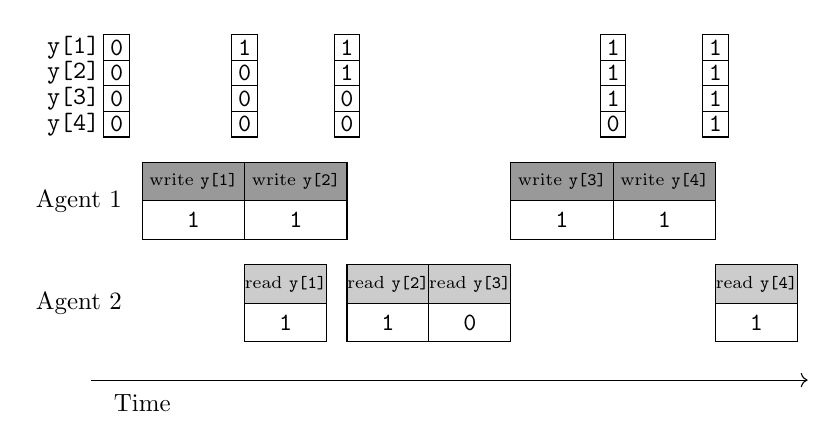
\begin{tikzpicture}[scale = 0.65, every node/.style={scale=0.9}]
\def\x{-1.6};
\def\y{7.25};
\fill[fill=white] ({\x},{\y}) rectangle ({\x+0.5},{\y+0.5}) node[pos=.5] {\texttt{y[4]}};
\fill[fill=white] ({\x},{\y+0.5}) rectangle ({\x+0.5},{\y+1}) node[pos=.5] {\texttt{y[3]}};
\fill[fill=white] ({\x},{\y+1}) rectangle ({\x+0.5},{\y+1.5}) node[pos=.5] {\texttt{y[2]}};
\fill[fill=white] ({\x},{\y+1.5}) rectangle ({\x+0.5},{\y+2}) node[pos=.5] {\texttt{y[1]}};


\def\x{-0.75};
\def\y{7.25};
\draw[] ({\x},{\y}) rectangle ({\x+0.5},{\y+0.5}) node[pos=.5] {\texttt{0}};
\draw[] ({\x},{\y+0.5}) rectangle ({\x+0.5},{\y+1}) node[pos=.5] {\texttt{0}};
\draw[] ({\x},{\y+1}) rectangle ({\x+0.5},{\y+1.5}) node[pos=.5] {\texttt{0}};
\draw[] ({\x},{\y+1.5}) rectangle ({\x+0.5},{\y+2}) node[pos=.5] {\texttt{0}};


\def\x{1.75};
\def\y{7.25};
\draw[] ({\x},{\y}) rectangle ({\x+0.5},{\y+0.5}) node[pos=.5] {\texttt{0}};
\draw[] ({\x},{\y+0.5}) rectangle ({\x+0.5},{\y+1}) node[pos=.5] {\texttt{0}};
\draw[] ({\x},{\y+1}) rectangle ({\x+0.5},{\y+1.5}) node[pos=.5] {\texttt{0}};
\draw[] ({\x},{\y+1.5}) rectangle ({\x+0.5},{\y+2}) node[pos=.5] {\texttt{1}};


\def\x{3.75};
\def\y{7.25};
\draw[] ({\x},{\y}) rectangle ({\x+0.5},{\y+0.5}) node[pos=.5] {\texttt{0}};
\draw[] ({\x},{\y+0.5}) rectangle ({\x+0.5},{\y+1}) node[pos=.5] {\texttt{0}};
\draw[] ({\x},{\y+1}) rectangle ({\x+0.5},{\y+1.5}) node[pos=.5] {\texttt{1}};
\draw[] ({\x},{\y+1.5}) rectangle ({\x+0.5},{\y+2}) node[pos=.5] {\texttt{1}};



\def\x{8.95};
\def\y{7.25};
\draw[] ({\x},{\y}) rectangle ({\x+0.5},{\y+0.5}) node[pos=.5] {\texttt{0}};
\draw[] ({\x},{\y+0.5}) rectangle ({\x+0.5},{\y+1}) node[pos=.5] {\texttt{1}};
\draw[] ({\x},{\y+1}) rectangle ({\x+0.5},{\y+1.5}) node[pos=.5] {\texttt{1}};
\draw[] ({\x},{\y+1.5}) rectangle ({\x+0.5},{\y+2}) node[pos=.5] {\texttt{1}};


\def\x{10.95};
\def\y{7.25};
\draw[] ({\x},{\y}) rectangle ({\x+0.5},{\y+0.5}) node[pos=.5] {\texttt{1}};
\draw[] ({\x},{\y+0.5}) rectangle ({\x+0.5},{\y+1}) node[pos=.5] {\texttt{1}};
\draw[] ({\x},{\y+1}) rectangle ({\x+0.5},{\y+1.5}) node[pos=.5] {\texttt{1}};
\draw[] ({\x},{\y+1.5}) rectangle ({\x+0.5},{\y+2}) node[pos=.5] {\texttt{1}};


        
%\node[text width=3cm] at (0.0,-2) {Agent 5};
%\node[text width=3cm] at (0.0,0) {Agent 4};
%\node[text width=3cm] at (0.0,2) {Agent 3};
\node[text width=3cm] at (0.0,4) {Agent 2};
\node[text width=3cm] at (0.0,6) {Agent 1};



%\def\n{-2};
%\def\m{10};
%\draw (\n, -3) -- (\m, -3);
%\draw (\n, -1) -- (\m, -1);
%\draw (\n, 1) -- (\m, 1);
%\draw (\n, 3) -- (\m, 3);
%\draw (\n, 5) -- (\m, 5);
%\draw (\n, 7) -- (\m, 7);

\def\n{0};
%\draw[style=dashed] (8.7, -2) -- (\m, -2);
%%\draw[style=dashed] (\n, 0) -- (\m, 0);
%%\draw[style=dashed] (\n, 2) -- (\m, 2);
%\draw[style=dashed] (7.7, 4) -- (\m, 4);
%\draw[style=dashed] (\n, 6) -- (2, 6);
%\node[style=rectangle,draw = black] at (1,0) {Agent 2 write};
\draw[fill=medgrey] (0,6) rectangle (2,6.75) node[pos=.5] {\scriptsize write \texttt{y[1]}};
\draw[fill=medgrey] (2,6) rectangle (4,6.75) node[pos=.5] {\scriptsize write \texttt{y[2]}};
\draw[fill=medgrey] (7.2,6) rectangle (9.2,6.75) node[pos=.5] {\scriptsize write \texttt{y[3]}};
\draw[fill=medgrey] (9.2,6) rectangle (11.2,6.75) node[pos=.5] {\scriptsize write \texttt{y[4]}};

\draw[] (0,5.25) rectangle (2,6) node[pos=.5] {\texttt{1}};
\draw[] (2,5.25) rectangle (4,6) node[pos=.5] {\texttt{1}};
\draw[] (7.2,5.25) rectangle (9.2,6) node[pos=.5] {\texttt{1}};
\draw[] (9.2,5.25) rectangle (11.2,6) node[pos=.5] {\texttt{1}};


\draw[fill=lightgrey] (2,4) rectangle (3.6,4.75) node[pos=.5] {\scriptsize  read \texttt{y[1]}};
\draw[fill=lightgrey] (4,4) rectangle (5.6,4.75) node[pos=.5] {\scriptsize  read \texttt{y[2]}};
\draw[fill=lightgrey] (5.6,4) rectangle (7.2,4.75) node[pos=.5] {\scriptsize  read \texttt{y[3]}};
\draw[fill=lightgrey] (11.2,4) rectangle (12.8,4.75) node[pos=.5] {\scriptsize  read \texttt{y[4]}};

\draw[] (2,3.25) rectangle (3.6,4) node[pos=.5] {\texttt{1}};
\draw[] (4,3.25) rectangle (5.6,4) node[pos=.5] {\texttt{1}};
\draw[] (5.6,3.25) rectangle (7.2,4) node[pos=.5] {\texttt{0}};
\draw[] (11.2,3.25) rectangle (12.8,4) node[pos=.5] {\texttt{1}};
\draw[->] (-1,2.5) -- (13,2.5);
\draw (0,2.4) node[below]{Time};

    \end{tikzpicture}
    \end{center}
Example of an inconsistent read. Agent 2 reads \texttt{y=[1,1,0,1]}, which was never an actual state of \texttt{y} in memory.
AC-FPI requires consistent reads within a single block but does allow inconsistent reads on \texttt{x} across different blocks.
(The delay within a single block must be the same, but different blocks may have different delays.)
\end{frame}



\begin{frame}
\frametitle{Race condition: inconsistent write}

\begin{center}
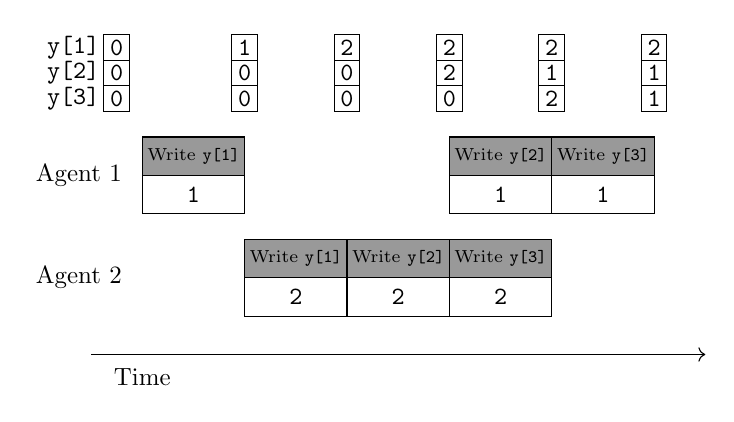
\begin{tikzpicture}[scale = 0.65, every node/.style={scale=0.9}]

\def\x{-1.6};
\def\y{6.75};
\fill[fill=white] ({\x},{\y+0.5}) rectangle ({\x+0.5},{\y+1}) node[pos=.5] {\texttt{y[3]}};
\fill[fill=white] ({\x},{\y+1}) rectangle ({\x+0.5},{\y+1.5}) node[pos=.5] {\texttt{y[2]}};
\fill[fill=white] ({\x},{\y+1.5}) rectangle ({\x+0.5},{\y+2}) node[pos=.5] {\texttt{y[1]}};


\def\x{-0.75};
\def\y{6.75};
\draw[] ({\x},{\y+0.5}) rectangle ({\x+0.5},{\y+1}) node[pos=.5] {\texttt{0}};
\draw[] ({\x},{\y+1}) rectangle ({\x+0.5},{\y+1.5}) node[pos=.5] {\texttt{0}};
\draw[] ({\x},{\y+1.5}) rectangle ({\x+0.5},{\y+2}) node[pos=.5] {\texttt{0}};


\def\x{1.75};
\def\y{6.75};
\draw[] ({\x},{\y+0.5}) rectangle ({\x+0.5},{\y+1}) node[pos=.5] {\texttt{0}};
\draw[] ({\x},{\y+1}) rectangle ({\x+0.5},{\y+1.5}) node[pos=.5] {\texttt{0}};
\draw[] ({\x},{\y+1.5}) rectangle ({\x+0.5},{\y+2}) node[pos=.5] {\texttt{1}};


\def\x{3.75};
\def\y{6.75};
\draw[] ({\x},{\y+0.5}) rectangle ({\x+0.5},{\y+1}) node[pos=.5] {\texttt{0}};
\draw[] ({\x},{\y+1}) rectangle ({\x+0.5},{\y+1.5}) node[pos=.5] {\texttt{0}};
\draw[] ({\x},{\y+1.5}) rectangle ({\x+0.5},{\y+2}) node[pos=.5] {\texttt{2}};


\def\x{5.75};
\def\y{6.75};
\draw[] ({\x},{\y+0.5}) rectangle ({\x+0.5},{\y+1}) node[pos=.5] {\texttt{0}};
\draw[] ({\x},{\y+1}) rectangle ({\x+0.5},{\y+1.5}) node[pos=.5] {\texttt{2}};
\draw[] ({\x},{\y+1.5}) rectangle ({\x+0.5},{\y+2}) node[pos=.5] {\texttt{2}};

\def\x{7.75};
\def\y{6.75};
\draw[] ({\x},{\y+0.5}) rectangle ({\x+0.5},{\y+1}) node[pos=.5] {\texttt{2}};
\draw[] ({\x},{\y+1}) rectangle ({\x+0.5},{\y+1.5}) node[pos=.5] {\texttt{1}};
\draw[] ({\x},{\y+1.5}) rectangle ({\x+0.5},{\y+2}) node[pos=.5] {\texttt{2}};


\def\x{9.75};
\def\y{6.75};
\draw[] ({\x},{\y+0.5}) rectangle ({\x+0.5},{\y+1}) node[pos=.5] {\texttt{1}};
\draw[] ({\x},{\y+1}) rectangle ({\x+0.5},{\y+1.5}) node[pos=.5] {\texttt{1}};
\draw[] ({\x},{\y+1.5}) rectangle ({\x+0.5},{\y+2}) node[pos=.5] {\texttt{2}};



\node[text width=3cm] at (0.0,4) {Agent 2};
\node[text width=3cm] at (0.0,6) {Agent 1};

%\node[style=rectangle,draw = black] at (1,0) {Agent 2 write};
\draw[fill=medgrey] (0,6) rectangle (2,6.75) node[pos=.5] {\scriptsize Write \texttt{y[1]}};
\draw[fill=medgrey] (6,6) rectangle (8,6.75) node[pos=.5] {\scriptsize Write \texttt{y[2]}};
\draw[fill=medgrey] (8,6) rectangle (10,6.75) node[pos=.5] {\scriptsize Write \texttt{y[3]}};

\draw[] (0,5.25) rectangle (2,6) node[pos=.5] {\texttt{1}};
\draw[] (6,5.25) rectangle (8,6) node[pos=.5] {\texttt{1}};
\draw[] (8,5.25) rectangle (10,6) node[pos=.5] {\texttt{1}};


\draw[fill=medgrey] (2,4) rectangle (4,4.75) node[pos=.5] {\scriptsize Write \texttt{y[1]}};
\draw[fill=medgrey] (4,4) rectangle (6,4.75) node[pos=.5] {\scriptsize Write \texttt{y[2]}};
\draw[fill=medgrey] (6,4) rectangle (8,4.75) node[pos=.5] {\scriptsize Write \texttt{y[3]}};

\draw[] (2,3.25) rectangle (4,4) node[pos=.5] {\texttt{2}};
\draw[] (4,3.25) rectangle (6,4) node[pos=.5] {\texttt{2}};
\draw[] (6,3.25) rectangle (8,4) node[pos=.5] {\texttt{2}};

\draw[->] (-1,2.5) -- (11,2.5);
\draw (0,2.4) node[below]{Time};


    \end{tikzpicture}
    \end{center}

Example of an inconsistent write.
The two writes of Agents 1 and 2 partially overwrite each other, and \texttt{y=[2,1,1]} is the resulting state.
An inconsistent write can occur when multiple agents attempt to concurrently write to the same block. 
% We enforce exclusive access to prevent inconsistent writes.
\end{frame}



\begin{frame}[fragile]
\frametitle{Race condition: inconsistency between \texttt{x} and \texttt{y}}
% Inconsistency between \verb|x| and \verb|y| is another possible race condition.
For this method to be an instance of ARock, the \verb|x| and \verb|y| that an agent reads must be related through the relationship \verb|y=A*x|.
This may fail to be hold if \verb|x| and \verb|y| are updated separately.
We can prevent this by enforcing exclusive  access for the whole \verb|(x,y)| pair:
% // p agents run the while loop asynchronously
% // x, y, and s in shared memory
\begin{lstlisting}
WHILE (not converged)
  1. Select i from Uniform{1,2,...,m}
  2. Read x,y
  3. Compute s[i] = eta*S[i](x) using y
  4. dy[i] = A[:,i]*s[i]
  5. Acquire exclusive access to (x,y)
  6. Read y and write y = y - dy[i]
     Read x[i] and write x[i] = x[i] - s[i]
  7. Release exclusive access to (x,y)
\end{lstlisting}


In some setups, exclusive access of Steps 5--7 can be a bottleneck.
% On a case-by-case basis, it may be possible to perform a specialized analysis to allow for inconsistency between \verb|x| and \verb|y|.
\end{frame}



\section{Parameter server framework}

\begin{frame}[fragile]
\frametitle{Parameter server framework}
The discussion so far was based on a \emph{shared memory system}, where multiple agents freely access variables stored in shared memory.
A single computer with a multi-core CPU is modeled well by a shared memory system. 
\medskip


In the \emph{parameter server framework} or \emph{server--worker framework}, a \emph{server}, or \emph{parameter server}, is a dedicated agent that collects, updates, and distributes variables over a network connected to \emph{workers}, the computational agents working in parallel.
\medskip

The parameter server can also perform minimal computation, so long as the server can keep up with the total throughput of the workers.
\medskip

A cluster of multiple computers connected to a central server node over a network is modeled well by the parameter server framework.

\end{frame}




\begin{frame}[fragile,plain]
\frametitle{Server--worker synchronous FPI}
One server and $m$ workers to compute $x^{k+1} = x^k - \eta \opS x^k$ synchronously:
\vspace{0.1in}

%The server initializes \verb|x| and runs
Server runs
\begin{lstlisting}
WHILE (not converged)
  Broadcast x to workers
  WHILE (not all indices processed)
    Pick any arrived, unprocessed s_i
    x[i] = x[i] - s_i
\end{lstlisting}
\vspace{0.1in}

Each worker runs (\verb|i = agent number|)
\begin{lstlisting}
WHILE (not converged)
  x << receive from server (wait until receive)
  s_i = eta*S[i](x)
  s_i >> server
\end{lstlisting}

\end{frame}



\begin{frame}[fragile]

This server--worker synchronous parallel algorithm has several potential sources of inefficiencies.
\begin{itemize}
    \item Between a broadcast and the first arrival of \verb!s_i!, the server is idle.
    \item Workers upload the \verb!s_i!'s around the same time, due to synchrony, and can cause a computational and communication bottleneck.
    \item A single \emph{straggler}, a worker taking significantly longer to process its work, can slow down the entire algorithm.
\end{itemize}

%it becomes likely for some \verb!s_i! to become the \emph{straggler} and delays the last arrival of \verb!s_i!.

\end{frame}



\begin{frame}[fragile,plain]
\frametitle{Server--worker asynchronous coordinate-update FPI}

An asynchronous implementation in the server--worker framework can avoid the inefficiencies of synchronization:
%The server initializes \verb!x! and runs

\vspace{0.1in}
Server runs
\begin{lstlisting}
// Queue holds s_i's. Queue is first-in-first-out
WHILE (not converged)
  WHILE (before next broadcast schedule)
    s_i =  Queue.pop() (wait until nonempty)
    x[i] = x[i] - s_i
  Broadcast(x)
\end{lstlisting}

\vspace{0.1in}
Each worker runs (\verb|i = agent number|)
\begin{lstlisting}
// Buffer holds only most recent x received 
// from server
WHILE (not converged)
  x << Buffer.read()
  s_i = eta*S[i](x)
  s_i >> server's queue
\end{lstlisting}

\end{frame}





\begin{frame}[fragile]

Server:
\begin{itemize}
    \item The \verb|Queue| stores the \verb!s_i! from workers.
    \item It broadcasts the latest \verb!x! at a certain interval.
    \item Between the broadcasts, the server processes the updates in the \verb|Queue| on a first-in-first-out basis.
    \item It must process the received \verb!s_i! sufficiently fast; otherwise, it cannot keep up with the workers and the \verb|Queue| will overflow.
\end{itemize}
\medskip

Worker:
\begin{itemize}
    \item Each worker has its \verb|Buffer| that holds the most recent copy of \verb|x| received from the server.
    \item Each worker uses its copy of \verb|x| to compute \verb!s_i!.
    \item Server broadcast should be sufficiently frequent so that the workers do not process the same \verb|x| too often.
\end{itemize}
\medskip

Inconsistent reads and writes do not arise in this setup, so there is no need for exclusive memory access.

\end{frame}



\begin{frame}[fragile]
\frametitle{Asynchronous server--worker AC-FPI}
We can still model this asynchronous algorithm with AC-FPI \eqref{eq:ac_fpi}:
\begin{itemize}
    \item Let $k$ increment whenever the server updates a block.
    \item Let $x^k$ be the copy of \verb!x! in the server memory after $k$th update.
    \item If the arrival times of \verb!s_1!,\dots,\verb!s_m! are $m$ independent and identical Poisson processes, then  $i(0),i(1),\dots$ is an IID random sequence.
\end{itemize}
In this case, this algorithm is an instance of ARock and we can apply Theorem~\ref{thm:ac-fpi}.
\bigskip

When $i(0),i(1),\dots$ is not an IID random sequence, Theorem~\ref{thm:ac-fpi} does not apply.
\end{frame}


\section{Methods}



\begin{frame}[fragile]
\frametitle{Methods}
\label{ss:async-methods}
We now present instances of AC-FPI on shared memory systems and on the parameter server framework.
\bigskip

The ARock assumptions are approximately, but not fully, satisfied by these algorithms.
%We point out and discuss which assumptions are satisfied and which are violated.

%When we solve large machine learning problems using many agents, we encounter the issue that they need to share variables, or model parameters in training, among other system states.
\end{frame}

\begin{frame}[fragile]
\frametitle{Asynchronous coordinate gradient descent}
Consider the problem
\[
\underset{x\in \reals^n}{\mbox{minimize}}\quad
  f\left(\sum_{i=1}^{m}A_{:,i}x_i-b\right) + \sum_{i=1}^{m}g_i(x_i),
\]
% where $g_1,\dots,g_m$ are CCP functions on $\reals^{n_1},\dots,\reals^{n_m}$, $f$ is a CCP function on $\reals^r$, $b\in \reals^r$, and
where
\[
A=\begin{bmatrix}
A_{:,1}&A_{:,2}&\cdots&A_{:,m}
\end{bmatrix}
\in
\reals^{r\times n}.
\]
\medskip

Assume for simplicity that we have $p=m$ agents.
% (If we have more blocks than agents, we can consolidate the $m$ blocks into $p$ groups.)
\medskip

Assume the $i$th agent has access to $x_i^k$, $\prox_{\alpha g_i}$, $A_{:,i}$, and $\nabla {f}$, for $i=1,\dots,m$.
% Assign $x_1^k,\dots,x_m^k$ to the $m$ agents.

\end{frame}

\begin{frame}[fragile]
The RC-FPI with the FBS operator is
\begin{align*}
  x^{k+1}_{i(k)} & = \prox_{\alpha g_{i(k)}}\left( x^{k}_{i(k)} - \alpha A^\intercal_{:,i(k)}\nabla {f} (y^k)  \right)\\
  y^{k+1}&=y^k+A_{:,i(k)}(x^{k+1}_{i(k)}-x^{k}_{i(k)}),
\end{align*}
where we initialize $y^{0}=Ax^0-b$.
The corresponding AC-FPI is
\begin{align*}
  s^k_{i(k)}&=\eta\left(\hat{x}^k_{i(k)}-\prox_{\alpha g_{i(k)}}\left( \hat{x}^{k}_{i(k)} - \alpha A^\intercal_{:,i(k)}\nabla {f} (\hat{y}^k)  \right)\right)\\
  x^{k+1}_{i(k)} & = x^k_{i(k)}-s^k_{i(k)}\\
  y^{k+1}&=y^k-A_{:,i(k)}s^k_{i(k)},
\end{align*}
where
\[
\hat{x}^{k}_{i(k)}=x^{k-d_{i(k)}(k)}_{i(k)},\qquad
\hat{y}^k=
A_{:,1}x^{k-d_{1}(k)}_{1}+\dots+A_{:,m}x^{k-d_{m}(k)}_{m}.
\]
% (Note that the blocks $x_1^k,\dots,x_m^k$ interact through the $y^k$ variable.)




% \begin{align*}
%   & \text{local}~(x_{I_j}',y') \gets (x,y)\\
%   & x'_{I_j} \gets \prox_{\alpha g_{I_j}}\left( x_{I_j} - \alpha A^\intercal_{:,I_j} \nabla{f} (y')\right)\\
%   & \text{acquire lock for~}(x_{I_j},y)\\
%   & \text{add}~ \eta A(x'_{I_j}-x_{I_j})~\text{to}~y\\
%   & \text{add}~ \eta(x'_{I_j}-x_{I_j}) ~\text{to}~x_{I_j}\\
%   & \text{release lock}.
% \end{align*}
% This is an ARock special case.
% Suppose $A$ has $m$ rows and $n$ columns, $m<n$, and we use $p$ agents, $p<m$. Assign roughly $n/p$ columns of $A$ and the corresponding entries of $x$ to each agent. This partitions $\{1,\dots,\}$ to $I_1,\dots,I_p$. Each agent $j=1,\dots,p$ holds $A_{:,I_j}$ and $x_{I_j}$. Introduce a parameter server to maintain $y = Ax-b$.

\end{frame}

\begin{frame}[fragile]


In a shared memory system, we can implement AC-FPI with
\begin{lstlisting}
// Shared memory code
// Initialize x=0, y=-b
// Pr_i = prox_{alpha*g_i}, G_f = gradient of f
WHILE (not converged) {
  //i = agent number
  Read y
  s[i] = eta*(x[i]-Pr_i(x[i]-alpha*A[:,i]'*G_f(y)))
  del[i] = -A[:,i]*s[i]
  Acquire exclusive access to y
  y = y + del[i]
  Release exclusive access to y
  x[i] = x[i] - s[i]
}
\end{lstlisting}
The momentary inconsistency between \verb!y! and \verb!x[i]! (after \verb!y! is updated but before \verb!x[i]! is updated) makes no difference to other agents since each \verb!x[i]! is read and updated by agent $i$ only. Effectively, \verb!y! and \verb!x[i]! are effectively updated simultaneously. But, staleness may still exist.


\end{frame}

\begin{frame}[fragile]
In a parameter server framework, we can implement AC-FPI with the server running
\begin{lstlisting}
// Server code
// Initialize y=-b
WHILE (not converged) {
  WHILE (before next broadcast schedule)
    IF Queue is empty, THEN wait until nonempty
    y = y + Queue.pop() 
  Broadcast(y)
}
\end{lstlisting}
% \begin{align*}
%   &y  \gets y + \sum_{i\in \text{receive buffer}}\Delta_i\\
%   &\text{broadcast}~ y
% \end{align*}
and the $m$ workers running (next slide)
\end{frame}

\begin{frame}[fragile]
\begin{lstlisting}
// Worker code
// Initialize x(1)=...=x(m)=0
// Pr_i = Prox_{alpha*g_i}, G_f = gradient of f
WHILE (not converged) {
  // i = agent number
  y << last received from server
  s_i = eta*(x_i-Pr_i(x_i-alpha*A[:,i]'*G_f(y)))
  (-A[:,i]*s_i) >> server's Queue
  x_i = x_i - s_i
}
\end{lstlisting}
\medskip

The value of \verb|y| received from the parameter server may be inconsistent with \verb|x| if the parameter server has not yet processed the worker's previous upload. For a means to ensure consistency, see Exercise~6.3.
\medskip

If each agent always updates the same block, the independence assumption does not hold even if all agents are equally powerful and the computational costs of all blocks are identical.
See Exercise 6.1.

\end{frame}








\begin{frame}[fragile]
\frametitle{Asynchronous ADMM}
Consider the optimization problem
\begin{align*}
\underset{x\in \reals^n}{\mbox{minimize}} \quad \frac{1}{m}\sum_{i=1}^{m} f_i(x) + g(x).
\end{align*}
We recast this problem into
\begin{align}\
\begin{array}{ll}
  \underset{x_1,\dots,x_m,y\in \reals^n}{\mbox{minimize}} & \frac{1}{m}\sum_{i=1}^{m} f_i(x_i) + g(y)\\
  \mbox{subject to} &~
  \underbrace{\begin{bmatrix}
          I & 0 & \dots & 0 \\
          0 & I & \dots & 0 \\
           &  & \ddots & \\
          0 & 0 & \dots & I
        \end{bmatrix}}_{=A}
        \begin{bmatrix}
          x_1 \\
          x_2 \\
          \vdots \\
          x_m
        \end{bmatrix}
        -
        \underbrace{
        \begin{bmatrix}
          I \\
          I \\
          \vdots \\
          I
        \end{bmatrix}}_{=B}
        y
        = 0.
        \end{array}
\end{align}
Define $f(x_1,\dots,x_m)=(1/m)(f_1(x_1)+\dots+f_m(x_m))$.
% \[
% f(x_1,\dots,x_m)=\frac{1}{m}\sum_{i=1}^{m} f_i(x_i).
% \]
As we did in \S3.2, consider the dual problem
\[
\begin{array}{ll}
  \underset{\nu}{\mbox{minimize}} & \underbrace{f^*(-A^\intercal \nu)}_{\tilde{f}(\nu)}+\underbrace{g^*(-B^\intercal \nu)}_{\tilde{g}(\nu)}.
  \end{array}
\]
%where $\tilde{f}(\nu)=f^*(-A^\intercal \nu)$ and $\tilde{g}(\nu)=g^*(-B^\intercal \nu)$.
%We follow the analysis of \S\ref{s:dualization-technique}.
\end{frame}


\begin{frame}[fragile]

The PRS operator (2.14) applied to the dual problem is
\[
  w^{k+1} = (2\prox_{\alpha \tilde{f}}-\opI)(2\prox_{\alpha \tilde{g}} -\opI)w^k.
\]
The FPI with the PRS operator averaged by $\eta\in(0,1)$ is
\begin{align*}
  y^{k+1} & = \argmin_{y\in \reals^n} \left\{g(y)- y^\intercal\sum_{j=1}^{m}w_j^k  + \frac{\alpha m}{2}\|y\|^2\right\}  \\
  %y^k & = \prox_{g/(\alpha m)}\left(  \frac{1}{\alpha m}\sum_{i=1}^{m}z_i^k  \right)\\
  %\nu_{i}^{k+1/2} & = z^k_{i} - \alpha y^k\\
  x^{k+1}_{i} & = \argmin_{x\in \reals^n}  \left\{\frac{1}{m}f_{i}(x) + x^\intercal\left(w^k_i-2\alpha y^{k+1}\right) + \frac{\alpha}{2}\|x\|^2  \right\}\quad\text{for }i=1,\dots,m\\
  %x^k_{i} & =\prox_{f_i/\alpha}\left(\frac{1}{\alpha}z^k_i-2 y^k  \right)\\
  %\nu_{i}^{k+1} & = 2 \nu_{i}^{k+1/2} -  z^k_{i} + \alpha x^k_{i},\\
  w^{k+1}_i&=w^k_i+2\eta\alpha(x^{k+1}_i-y^{k+1})\quad\text{for }i=1,\dots,m.
\end{align*}
\end{frame}


\begin{frame}[fragile]
%{\color{blue} XXX Replace $\psi^k$ in \S\ref{s:dualization-technique} by $w^k$ and multiply its update step size by $2\eta$ XXX}
With the change of variables $w^k=\alpha u^k$ and $\rho=1/(\alpha m)$, we get
\begin{align*}
  %y^k & = \argmin_{y\in \reals^n} \left\{g(y)- y^\intercal\sum_{i=1}^{m}z_i^k  + \frac{\alpha m}{2}\|y\|^2\right\}  \\
  y^{k+1} & = \prox_{\rho g}\left(  \frac{1}{ m}\sum_{j=1}^{m}u_j^k  \right)\\
  %\nu_{i}^{k+1/2} & = z^k_{i} - \alpha y^k\\
  %x^k_{i} & \in \argmin_{x\in \reals^n}  \left\{f_{i}(x) + x^\intercal\left(z^k_i-2\alpha y^k\right) + \frac{\alpha}{2}\|x\|^2  \right\}\quad\text{for }i=1,\dots,m\\
  x^{k+1}_{i} & =\prox_{\rho f_i}\left(2 y^{k+1}-u^{k}_i \right)\quad\text{for }i=1,\dots,m\\
  %\nu_{i}^{k+1} & = 2 \nu_{i}^{k+1/2} -  z^k_{i} + \alpha x^k_{i},\\
  u^{k+1}_i&=u^k_i+2\eta(x^{k+1}_i-y^{k+1})\quad\text{for }i=1,\dots,m.
\end{align*}
The corresponding AC-FPI is
\begin{align*}
  y^{k+1} & = \prox_{\rho g}\left(  (1/m)\hat{u}_\mathrm{sum}^k  \right)\\
  x^{k+1}_{i(k)} & =\prox_{\rho f_{i(k)}}\left(2 y^{k+1}-\hat{u}^k_{i(k)} \right)\\
  u^{k+1}_{i(k)}&=u^k_{i(k)}+2\eta(x^{k+1}_{i(k)}-y^{k+1})
  %u_\mathrm{sum}^{k+1}&=u_\mathrm{sum}^{k}+2\eta(x^k_{i(k)}-y^k)
\end{align*}
where
\[
\hat{u}^k_{i(k)}
=u^{k-d_{i(k)}(k)}_{i(k)},
\qquad
\hat{u}_\mathrm{sum}^k=u_1^{k-d_1(k)}+\dots+u_m^{k-d_m(k)}.
\]
\end{frame}


\begin{frame}[fragile]
\frametitle{Asynchronous ADMM server--worker implementation}
%Consider a parameter server framework.
Assume
\begin{itemize}
    \item there are $p=m$ workers,
    \item each $i$th worker has access to $u_i^k$ and $\prox_{ f_i/\alpha}$, and
    \item the server has access to $\prox_{ g/(\alpha m)}$.
\end{itemize}
\medskip

We can implement ARock with the server running
\begin{lstlisting}
// Parameter server code
// Initialize u_sum=0
WHILE (not converged) {
  WHILE (before next broadcast schedule)
    IF Queue is empty, THEN wait until nonempty
    s = Queue.pop()
    u_sum = u_sum + s
  y = Prox_{rho*g}(u_sum/m)
  Broadcast(y)
}
\end{lstlisting}
\end{frame}


\begin{frame}[fragile]
and each of the $m$ workers running
\begin{lstlisting}
// Worker code
// Initialize u[1]=...=u[m]=0
WHILE (not converged) {
  //i = agent number
  y << last received from server
  x_i = Prox_{rho*f_i}(2*y-u_i)
  2*eta*(x_i-y) >> server's Queue
  u_i = u_i + 2*eta*(x_i - y)
}
\end{lstlisting}
\medskip

The discussions on consistency and the independence assumption for the previous example still apply to this example.

\end{frame}


\section{Exclusive memory access}



\begin{frame}
\frametitle{Exclusive memory access}
We now discuss how to implement exclusive memory access using atomic operations and mutual exclusion locks.
We limit the discussion at a superficial level, just enough to provide clarity on the behavior and the implementation of AC-FPI.

\bigskip

For a more thorough discussion on the lower-level considerations of concurrent programming, we refer to readers to standard resources.
\end{frame}


\begin{frame}
\frametitle{Atomic operations}
An operation of a computational agent is \emph{atomic} if the whole operation is guaranteed to complete without interruption (or never start) in the presence of contention from other agents; if an atomic operation consists of multiple steps, other agents will not observe intermediate results. 
\medskip

In most modern systems, reading and writing a single number (represented as a 32- or 64-bit floating-point number) is an atomic operation.
\end{frame}


\begin{frame}[fragile]

Consider the case where all blocks are single coordinates, i.e., $m=n$ and $n_1=\dots= n_m=1$.
Then we can implement the AC-FPI as follows.
\begin{lstlisting}
// p agents run the while loop asynchronously
WHILE (not converged) {
  1. Select i from Uniform{1,2,...,m}
  2. for j = 1,...,m
       read x[j]
  3. Compute s[i] = -eta*S[i](x)
  4. x[i] += s[i] (atomic with compare-and-swap)
}
\end{lstlisting}
%Since reading a single number of atomic, 
In Step 2, each coordinate \verb|x[j]| is read consistently though different coordinates may have different delays.
\smallskip

Step 4 uses the \emph{increment} operator \verb|+=|.  \verb|a+=b| implies \verb|a=a+b|.
\smallskip

The increment operator reads from \verb|a| and \verb|b|, computes the sum, and writes to \verb|a|.
Despite several erroneous claims in the asynchronous optimization literature, \verb|+=| is often \emph{not} atomic in many CPUs and GPUs;
when multiple agents simultaneously increment the same variable, one agent can overwrite another's increment.
\end{frame}


\begin{frame}[fragile]
\frametitle{Atomic increment by compare-and-swap}
The \emph{atomic increment} can be implemented via compare-and-swap:
\begin{lstlisting}
// atomic a += b
do {
  old <- a
} while ( !compare_and_swap(a, old, old+b) )
\end{lstlisting}
\end{frame}


\begin{frame}[fragile]
\frametitle{The compare-and-swap instruction}

Most modern CPUs and GPUs support the \emph{compare-and-swap} instruction as an atomic operation. It corresponds to:
\begin{lstlisting}
// atomic execution
// input num is passed by reference and is
// modifiable
function compare_and_swap(num, old, new) {
  if num != old
    return false
  num <- new
  return true
}
\end{lstlisting}
\medskip

If \verb|num| is equal to \verb|old|, then write \verb|new| to \verb|num| and return \verb|true|; otherwise do nothing and return \verb|false|.
\end{frame}


\begin{frame}[fragile]{AC-FPI when block has multiple coordinates}

This algorithm is no longer valid:
\begin{lstlisting}
// p agents run the while loop asynchronously
WHILE (not converged) {
  1. Select i from Uniform{1,2,...,m}
  2. for j = 1,...,m
       read block x[j]
  3. Compute s[i] = -eta*S[i](x)
  4. x[i] += s[i] (atomic with compare-and-swap)
}
\end{lstlisting}
\medskip

The reads of Step 2 are no longer guaranteed to be consistent as it is possible for \verb|x[j]| to be updated by another agents while it is being read.
\medskip

Moreover, the atomic increment via compare-and-swap is no longer possible as compare-and-swap is usually only supported for data types of size 64-bits or smaller.
\end{frame}



\begin{frame}[fragile]
\frametitle{Mutual exclusion lock}
A \emph{mutual exclusion lock} or \emph{mutex} comes with a \emph{lock} and an \emph{unlock} methods and
is \emph{acquired} by at most one agent at any given time. 
\medskip

An agent acquires a mutex with the \verb|lock()| method. An agent \emph{releases} a mutex with the \verb|unlock()| method.
\medskip

If the mutex is available, \verb|lock()| returns immediately and acquires the mutex.
Otherwise (if another agent has locked the mutex and has not yet unlocked it) \verb|lock()| waits until the mutex becomes available and then acquires the mutex.
\medskip

The \verb|unlock()| method returns immediately. If other agents are waiting to acquire the mutex, then one of the waiting agents acquire the mutex upon the unlock.

%Mutexes can be implemented using the compare-and-swap operation, although it is usually better to rely on implementations provided by standard libraries.
\end{frame}



\begin{frame}[fragile]
\frametitle{Mutual exclusion lock}
An inefficient way to implement exclusive access in AC-FPI is:
\begin{lstlisting}
// AC-FPI with one mutex. Inefficient!
WHILE (not converged)
  1. Select i from Uniform{1,2,...,m}
  2. mutex.lock()
     Read x
     mutex.unlock()
  3. Compute s[i] = eta*S[i](x)
  4. mutex.lock()
     x[i] = x[i] - s[i]
     mutex.unlock()
\end{lstlisting}
%With this locking mechanism, the delays of all blocks are uniform.
\end{frame}


\begin{frame}[fragile]
\frametitle{Mutual exclusion lock}


Rather it is more efficient to use separate mutexes for all blocks:
\begin{lstlisting}
// AC-FPI with mutex for each block
WHILE (not converged)
  1. Select i from Uniform{1,2,...,m}
  2. for j = 1,...,m
       mutex[j].lock()
       read x[j]
       mutex[j].unlock()
  3. Compute s[i] = eta*S[i](x)
  4. mutex[i].lock()
     x[i] = x[i] - s[i]
     mutex[i].unlock()
\end{lstlisting}
This mechanism ensures the reads and writes of all blocks are consistent while allowing multiple agents to concurrently operate on separate blocks.
However, Step 2 is still inefficient as it prevents multiple agents from concurrently reading the same block.

%In Step 2, each block \verb|x[j]| is read consistently, although different blocks may have different delays.

\end{frame}

\begin{frame}[fragile,plain]
\frametitle{Readers-writers lock}
A \emph{readers-writers lock} allows concurrent access for reads while enforcing exclusive access for writes.
% The following class implements a readers-writers lock.
\begin{lstlisting}
class rw_lock:
  int b; mutex MUTEX_b; mutex MUTEX_W
  rw_lock(): b = 0 //constructor
  function read_lock():
    MUTEX_b.lock()
    b++
    If b==1, MUTEX_W.lock()
    MUTEX_b.unlock()
  function read_unlock():
    MUTEX_b.lock()
    b--
    If b==0, MUTEX_W.unlock()
    MUTEX_b.unlock()
  function write_lock():
    MUTEX_W.lock()
  function write_unlock():
    MUTEX_W.unlock()
\end{lstlisting}

\end{frame}

\begin{frame}[fragile]
    Variable \verb|b| keeps track of the number of concurrent reads. Each call to \verb|read_lock()| increases \verb|b| by 1, and each call to \verb|read_unlock()| decreases \verb|b| by 1. \verb|MUTEX_b| ensures only one reader can modify \verb|b| at any time.
    \medskip

    When an agent calls \verb|read_lock()|, if it increases \verb|b| from 0 to 1, it will also try to acquire \verb|MUTEX_W|. %When an agent calls \verb|read_unlock()|, only if it decrements \verb|b| to 0, will it release \verb|MUTEX_W|.
    \medskip
    
    When \verb|b| $\ge 1$, \verb|MUTEX_W| is locked and there are one or more readers. A writer must wait until \verb|b| returns 0, that is, there are no more readers.
    \medskip

    When \verb|MUTEX_W| is locked by a writer, all readers must wait.
    
\end{frame}

\begin{frame}[fragile]
\frametitle{AC-FPI with readers--writers locks}
\begin{lstlisting}
// AC-FPI with readers-writers locks
WHILE (not converged)
  1. Select i from Uniform{1,2,...,m}
  2. for j = 1,...,m
       rw_lock[j].read_lock()
       read x[j]
       rw_lock[j].read_unlock()
  3. Compute s[i] = eta*S[i](x)
  4. rw_lock[i].write_lock()
     x[i] = x[i] - s[i]
     rw_lock[i].write_unlock()
\end{lstlisting}
This mechanism ensures the reads and writes of all blocks are consistent, allows multiple agents to concurrently operate on separate blocks, and allows multiple agents to concurrently read from the same block.
\end{frame}

\begin{frame}

This implementation of the readers--writers locks prioritizes readers: if there are many readers, a writer must wait until there are no more readers. If there are many writers, a reader may acquire the lock while some other writers are waiting. 
\bigskip

To reduce the staleness as much as possible, one could use a readers-writers lock prioritizing writers. However, such locks are more complex and allow for less concurrency.
\end{frame}

\end{document}